\setdictum{%
  The goal is to buy as many iPads as possible during your lifetime.%
}{%
  In a talk at the 5th Workshop on\\Sparse Grids and Applications%
}

\longchapter{%
  Application 3: Dynamic Portfolio Choice Models%
}{%
  Application 3:\texorpdfstring{\\}{ }Dynamic Portfolio Choice Models%
}{%
  Application 3 -- Dynamic Portfolio Choice Models%
}
\label{chap:80finance}

\initial[lhang=0.06]{0.1em}{S}{urrogates based on B-splines on sparse grids}
can also be used for our third application,
which stems from finance.
In this application, we optimize financial decisions of an individual
over their lifetime in discrete time steps or iterations $t = 0, \dotsc, T$
(for example, years $t = 0, \dotsc, 80$, where $20+t$ is the age
of the individual), depending on internal and external factors.
There are three types of variables:

\begin{itemize}
  \item
  \term{State variables} $\state_t$
  such as the individual's wealth $\wealth_t$ and their income
  cannot be controlled directly by the individual.
  Instead, the individual's decisions may influence the value of
  state variables of future iterations.%
  \footnote{%
    The time $t$ can also be regarded as a state variable.%
  }
  
  \item
  \term{Policy variables} $\policy_t$
  such as consumption $\consume_t$ and the amount of stocks to buy or sell
  represent the investment decisions the individual can make in
  each iteration.
  They are subject to specific constraints
  (for instance, you cannot spend more money than you have,
  if you do not allow debts).
  
  \item
  \term{Stochastic variables} $\stochastic_t$
  such as return rates of stocks and inflation
  cannot be controlled by the individual at all.
  Therefore, statements about optimal investment conditions
  are usually made for expected values instead of exact values.
\end{itemize}

\noindent
We discretize the state space with a spatially adaptive sparse grid.
For each state grid point, an optimization problem over the policy
variables has to be solved, where the objective function depends
on the expected value over the stochastic variables.
By using B-splines as hierarchical basis functions,
the accuracy of the interpolants is increased and
the explicitly known gradients enable the usage of
gradient-based optimization methods, thus accelerating convergence.
The process is repeated for each time step,
which is possible due to the Bellman principle,
which implies that the objective functions
occurring at time $t$ depend on the interpolant of the next iteration $t+1$.
Hence, the problem has to be solved backward in time
via a scheme that closely resembles dynamic programming.

The outline of this chapter is as follows:
In \cref{sec:81models}, we formalize the framework of
dynamic portfolio choice models and describe our approach.
Afterwards, we explain in \cref{sec:82algorithms} the necessary algorithms
for implementing the solution of these models.
\Cref{sec:83problem} introduces the transaction costs problem
as an example application of the general framework presented
in \cref{sec:81models}.
Finally, in \cref{sec:84results}, we study numerical results.

This chapter is based on a collaboration with Prof.\ Dr.\ Raimond Maurer
and Peter Schober (both Goethe University Frankfurt, Germany).
In previous work, Peter Schober treated the solution of
dynamic portfolio choice models with piecewise linear basis functions
on spatially adaptive sparse grids \cite{Schober18Solving}.
The original contribution of this thesis is the introduction
of higher-order B-splines for the solution of these problems.
The author of this thesis contributed the methodology of
hierarchical B-splines and large parts of the implementation.
The contributions of the collaborators at Goethe University Frankfurt
are the financial models, the literature review of related work,
and the assessment of the quality of results.

\section{Solving the Bellman Equation}
\label{sec:81models}

\minitoc[-0.5mm]{76mm}{4}

\noindent
In this section, we give a mathematical framework for
dynamic portfolio choice models,
briefly mention related literature, and
explain where B-splines on sparse grids come into play.
\Cref{tbl:glossaryFinance} summarizes the symbols
that are introduced in this chapter.
Rust provides a more detailed introduction to
dynamic portfolio choice models \cite{Rust18Dynamic}.

\begin{table}
  \setnumberoftableheaderrows{0}%
  \newcommand*{\vph}{%
    \vphantom{\printnotationsymbol{\buysell}}%
  }%
  \newcommand*{\pnst}[1]{%
    \printnotationsymbol{#1}\vph&\printnotationtext{#1}%
  }%
  \newcommand*{\pnsta}[1]{%
    \printnotationsymbol{#1}\vph&\multicolumn{3}{l}{\printnotationtext{#1}}%
  }%
  \begin{tabular}{%
    >{\kern\tabcolsep}=l+l<{\kern4.5mm}+l<{\kern-1.5mm}+l%
    <{\kern4.5mm}+l<{\kern-1mm}+l<{\kern\tabcolsep}%
  }
    \toprulec
    \pnst{t}&            \pnst{\wealth}&      \pnst{\utilityfcn}\\
    \pnst{\state}&       \pnst{\consume}&     \pnst{\statefcn}\\
    \pnst{\policy}&      \pnst{\bond}&        \pnst{\valuefcn}\\
    \pnst{\stochastic}&  \pnsta{\cetvalueintp}\\
    \pnst{\riskav}&      \pnst{\stock}&       \pnst{\optpolicyfcn}\\
    \pnst{\patience}&    \pnst{\buysell}&     $\hat{({\cdot})}$&Normalized quantity\\
    \pnst{\bondreturn}&  \pnst{\stockreturn}& \pnst{\wealthratio}\\
    \pnst{\tac}&         \pnsta{\weightedeulererror}\\
    \bottomrulec
  \end{tabular}%
  \caption[Glossary for dynamic portfolio choice models]{%
    Glossary of the notation for dynamic portfolio choice models.%
  }%
  \label{tbl:glossaryFinance}%
\end{table}



\subsection{Bellman Equation}
\label{sec:811bellmanEquation}

\paragraph{Utility maximization}

\usenotation{t}
In the following, dynamic portfolio choice models aim to maximize the expected
\term{discounted time-additive utility} over the lifetime of the individual,
where the terminal utility is derived solemnly from consumption
(i.e., no inheritance motive).
If we neglect stochastic factors, then these models solve
\begin{equation}
  \label{eq:utilityMaximization}
  (\optpolicyfcn_0, \dotsc, \optpolicyfcn_T)
  = \vecargmax_{\policy_0, \dotsc, \policy_T}
  \sum_{t=0}^T \patience^t \utilityfcn(\consume_t(\state_t, \policy_t))
  \quad\text{s.t. specific constraints.}
\end{equation}
Here, $\state_t \in \clint{\*0, \*1} \subset \real^d$ and
$\policy_t \in \real^{m_{\policy}}$
are the state%
\footnote{%
  We assume that each state variable $\stateentry_{t,o}$ ($o = 1, \dotsc, d$)
  is bounded, since the state space will be discretized with sparse grids.
  Without loss of generality, we may then assume that
  $\state_t \in \clint{\*0, \*1}$.
  If some state variables are unbounded in reality,
  then extrapolation is necessary,
  which will be explained in \cref{sec:825interpolation}.%
}
and policy of time $t = 0, \dotsc, T$, respectively.
The constraints ensure that for instance, we do not spend more money
than we actually have.
Starting from a given initial state $\state_0$,
the state $\state_{t+1}$ of time $t+1$ can be computed from
$\state_0$ and $\policy_0, \dotsc, \policy_t$ with a
\term{state transition function} $(\state_t, \policy_t) \mapsto \state_{t+1}$.
As shown in \cref{fig:dynamicPortfolioChoice},
in each time step, a fraction of the available wealth is consumed
\term{(consumption $\consume_t$),}
which can be computed from the state $\state_t$ and the policy $\policy_t$.
The individuals rate the consumption with a \term{utility function}
$\utilityfcn(\consume_t)$.
A common choice for $\utilityfcn$ is the \term{\crra utility}
$\utilityfcn(\consume_t) \ceq c_t^{1-\riskav}/(1-\riskav)$
with the \term{risk aversion} $\riskav \in \real \setminus \{1\}$.
Positive and negative values of $\riskav$
correspond to risk-averse and risk-affine individuals, respectively.
The factor $\patience \in \pohint{0, 1}$ is the \term{patience}
or \term{time discount factor.}

\begin{SCfigure}
  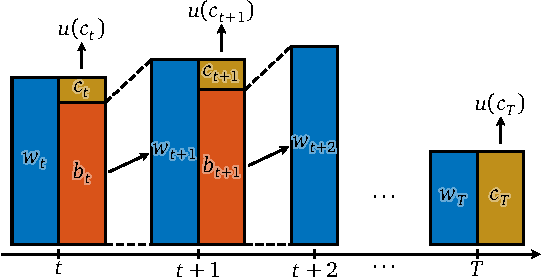
\includegraphics{dynamicPortfolioChoice_1}%
  \caption[Example of a dynamic portfolio choice model]{%
    Example of a dynamic portfolio choice model.
    The available wealth $\wealth_t$ is either
    invested into risk-free bonds ($\bond_t$) or consumed ($\consume_t$),
    resulting in utility $\utilityfcn(\consume_t)$.
    In the last time step $T$ \emph{(far right),}
    the optimal solution is to consume the whole wealth,
    if we do not take inheritance into account.%
  }%
  \label{fig:dynamicPortfolioChoice}%
\end{SCfigure}

\paragraph{Limitations of naive utility maximization}

When solving the utility maximization problem
in \cref{eq:utilityMaximization}, there are two issues.
First, solving \cref{eq:utilityMaximization} for all times $t$ at once
implies solving a $(T+1) m_{\policy}$-dimensional optimization problem,
which is usually computationally infeasible.
Second, \cref{eq:utilityMaximization} does not take stochastic variables
$\stochastic_t$ such as stock return rates into account.
These variables influence the state transition, i.e.,
$(\state_t, \policy_t, \stochastic_t) \mapsto \state_{t+1}$.
Consequently, $\state_{t+1}$ cannot be computed from $\state_0$ and
$\policy_0, \dotsc, \policy_t$ alone,
which complicates the solution of \cref{eq:utilityMaximization}
even for expected values.

\paragraph{Bellman principle}

To resolve the first issue,
Bellman's principle of optimality \cite{Bellman57Dynamic}
can be applied to problems like
\cref{eq:utilityMaximization} that are said to have
\term{optimal substructure.}
The principle states that the optimal policy for all times $t = 0, \dotsc, T$
is also optimal with respect to $t = 1, \dotsc, T$, i.e.,
{%
  \setlength{\abovedisplayskip}{6pt}%
  \begin{equation}
    \max_{\policy_0, \dotsc, \policy_T}
    \sum_{t=0}^T \patience^t \utilityfcn(\consume_t(\state_t, \policy_t))
    = \max_{\policy_0} \left(
      \utilityfcn(\consume_0(\state_0, \policy_0))
      + \patience \max_{\policy_1, \dotsc, \policy_T}
      \sum_{t=1}^T \patience^{t-1} \utilityfcn(\consume_t(\state_t, \policy_t))
    \right),
  \end{equation}%
}%
where we omitted the constraints for brevity.
The inner maximum problem over $\policy_1, \dotsc, \policy_T$
has the same structure as the problem on the \lhs.
With the \term{value function}
$\valuefcn_t\colon \clint{\*0, \*1} \to \real$,
$\valuefcn_t(\state_t) \ceq
\max_{\policy_t, \dotsc, \policy_T}
\sum_{t'=t}^T \patience^{t'-t}
\utilityfcn(\consume_{t'}(\state_{t'}, \policy_{t'}))$,
this can be rewritten as
{%
  \setlength{\belowdisplayskip}{9pt}%
  \begin{equation}
    \label{eq:simpleBellman}
    \valuefcn_0(\state_0)
    = \max_{\policy_0} \left(
      \utilityfcn(\consume_0(\state_0, \policy_0)) +
      \patience \valuefcn_1(\state_1)
    \right)
    \quad\text{s.t. specific constraints,}
  \end{equation}%
}%
where $\state_1$ is the result of the state transition
starting from $(\state_0, \policy_0)$.

\paragraph{General Bellman equation}

If we formulate \cref{eq:simpleBellman} for arbitrary times $t$ and
consider constraints, state transition, and stochastic variables,
we obtain the \term{Bellman equation:}
\begin{subequations}
  \setlength{\abovedisplayskip}{9pt}%
  \label{eq:generalBellman}
  \begin{gather}
    \valuefcn_t(\state_t)
    = \max_{\policy_t} \left(
      \utilityfcn(\consume_t(\state_t, \policy_t)) +
      \patience \expectation[t]{
        \valuefcn_{t+1}(\statefcn_t(\state_t, \policy_t, \stochastic_t))
      }
    \right),\quad
    t = 0, \dotsc, T,\\[-2mm]
    \policy_t \in \real^{m_{\policy}}\;\;\text{s.t.}\;\;
    \ineqconfun_t(\state_t, \policy_t) \le \*0,
  \end{gather}
\end{subequations}
where $\valuefcn_{T+1} :\equiv 0$ for simplicity,
$\statefcn_t\colon \clint{\*0, \*1} \times \real^{m_{\policy}} \times
\stochdomain \to \clint{\*0, \*1}$,
$(\state_t, \policy_t, \stochastic_t) \mapsto \state_{t+1}$,
is the \term{state transition function,}
$\ineqconfun_t\colon \clint{\*0, \*1} \times \real^{m_{\policy}} \to
\real^{m_{\ineqconfun}}$ is the \term{constraint function,} and
\begin{equation}
  \expectation[t]{
    \valuefcn_{t+1}(\statefcn_t(\state_t, \policy_t, \stochastic_t))
  }
  \ceq \int_{\stochdomain}
  \valuefcn_{t+1}(\statefcn_t(\state_t, \policy_t, \stochastic_t))
  P_{t,\stochastic}(\stochastic_t) \diff{}\stochastic_t
\end{equation}
with the probability density function
$P_{t,\stochastic}\colon \stochdomain \to \nonnegreal$ of $\stochastic_t$.%
\footnote{%
  While the state $\state_t \in \clint{\*0, \*1}$
  is continuous in this thesis,
  \term{Markov-chain discrete states} $\discrstate_t \in \discrstdomain$
  such as alive/dead
  (i.e., $\discrstdomain$ is the Cartesian product of finite sets)
  can be incorporated into \eqref{eq:generalBellman}.
  The objective function of $\valuefcn_t(\state_t, \discrstate_t)$ then equals
  $\utilityfcn(\consume_t(\state_t, \discrstate_t, \policy_t)) +
  \patience \expectation[t]{
    \valuefcn_{t+1}(\statefcn_t(\state_t, \discrstate_t,
    \policy_t, \stochastic_t), \discrstate_{t+1}) \mid \discrstate_t
  }$.%
}
We denote the location of the maximum of \eqref{eq:generalBellman}
as the optimal policy $\optpolicyfcn_t$,
which may be regarded as a function
$\optpolicyfcn_t\colon \clint{\*0, \*1} \to \real^{m_{\policy}}$,
$\state_t \mapsto \optpolicyfcn_t(\state_t)$.

\paragraph{Dynamic programming scheme}

The Bellman equation \eqref{eq:generalBellman} can be solved
backwards in time with a dynamic programming scheme.
Starting from the solution $\valuefcn_T$ and $\optpolicyfcn_T$
of time $T$, which is determined by maximizing the utility
for the terminal time step,
we can determine $\valuefcn_t$ and $\optpolicyfcn_t$
from $\valuefcn_{t+1}$ and $\optpolicyfcn_{t+1}$
for $t = T - 1,\, T - 2,\, \dotsc,\, 0$ with the Bellman equation.
This way, we only have to solve $T+1$ separate $m_{\policy}$-dimensional
optimization problems instead of a single large
$(T+1) m_{\policy}$-dimensional problem.
Often, the terminal solutions $\valuefcn_T$ and $\optpolicyfcn_T$
are explicitly known.
In our case, the optimal terminal solution is
to consume the whole wealth $\wealth_T$
(see \cref{fig:dynamicPortfolioChoice}).

\paragraph{Implementation and interpolation}

For the implementation of \eqref{eq:generalBellman},
we discretize the state space $\clint{\*0, \*1}$ into
$\ngp_t$ grid points $\state_t^{(k)}$, $k = 1, \dotsc, \ngp_t$,
and we tabulate the values of $\valuefcn_t$ and $\optpolicyfcn_t$
at $\state_t^{(k)}$ for all $t = 0, \dotsc, T$ and $k = 1, \dotsc, \ngp_t$.
However, in general, the next state
$\statefcn_t(\state_t^{(k)}, \policy_t, \stochastic_t)$ does not correspond
to a grid point $\state_{t+1}^{(k')}$,
which means that we cannot lookup the value of $\valuefcn_{t+1}$
at $\statefcn_t(\state_t^{(k)}, \policy_t, \stochastic_t)$.
Therefore, we have to interpolate $\valuefcn_{t+1}$
at the grid points, obtaining the interpolant $\valueintp_{t+1}$
as a result:
\begin{equation}
  \label{eq:gridBellman}
  \valueintp_t(\state_t^{(k)})
  = \max_{\policy_t} \left(
    \utilityfcn(\consume_t(\state_t^{(k)}, \policy_t)) +
    \patience \expectation[t]{
      \valueintp_{t+1}(\statefcn_t(\state_t^{(k)}, \policy_t, \stochastic_t))
    }
  \right),\quad
  k = 1, \dotsc, \ngp_t,
\end{equation}
where $\valueintp_{T+1} :\equiv 0$ for simplicity.
As $\valueintp_{t+1}$ on the \rhs is only an approximation to
$\valuefcn_{t+1}$, the values $\valueintp_t(\state_t^{(k)})$
on the \lhs are approximations, too.
Since we are mainly interested in the optimal policy decisions
$\optpolicyfcn_t$, we have to interpolate them as well, i.e.,
\begin{equation}
  \optpolicyintp_t(\state_t^{(k)})
  = \vecargmax_{\policy_t} \left(
    \utilityfcn(\consume_t(\state_t^{(k)}, \policy_t)) +
    \patience \expectation[t]{
      \valueintp_{t+1}(\statefcn_t(\state_t^{(k)}, \policy_t, \stochastic_t))
    }
  \right).
\end{equation}
Note that the employed grids for $\optpolicyintp_t$
may be different from the grids for $\valueintp_t$.



\subsection{Solution with B-Spline Surrogates on Sparse Grids}
\label{sec:812surrogates}

\paragraph{Sparse grids for dynamic models and related work}

As interpolation approaches for $\valuefcn_t$ based on full grids
suffer from the curse of dimensionality,
we want to use interpolation on spatially adaptive sparse grids instead.
Recently, sparse grids have found increasing interest in the
solution of dynamic models in finance
\multicite{Brumm17Using,Judd14Smolyak,Schober18Solving,Winschel10Solving}.
For example in \cite{Brumm17Using},
discrete choices in the value iteration are computed
using piecewise linear basis functions on spatially adaptive sparse grids.
Schober employs spatially adaptive sparse grids
for the interpolation of dynamic portfolio choice models,
but uses piecewise linear basis functions \cite{Schober18Solving}.
Judd et al.\ use global polynomials
on sparse Clenshaw--Curtis grids for the interpolation of
higher-dimensional economic models \cite{Judd14Smolyak}.

\paragraph{B-splines on sparse grids for dynamic portfolio choice models}

The shortcomings of the two approaches of piecewise linear functions
\multicite{Brumm17Using,Schober18Solving} or global polynomials
\cite{Judd14Smolyak} are evident:
Piecewise linear functions are not continuously differentiable,
impeding convergence of interpolation errors
(see \cref{sec:541interpolation}) and prohibiting the use
of gradient-based optimization methods to solve \cref{eq:gridBellman}.
The reason for the latter statement is that gradient-based optimizers require
the derivatives of the objective function of \cref{eq:gridBellman}
with respect to the entries $\policyentry_{t,j}$ of $\policy_t$
($j = 1, \dotsc, m_{\policy}$), i.e.,
\begin{equation}
  \begin{split}
    &\utilityfcn'(\consume_t(\state_t^{(k)}, \policy_t))
    \partialderiv{\partialdiff{}\policyentry_{t,j}}{c_t}\paren{
      \state_t^{(k)}, \policy_t
    }\\
    &{} + \patience \expectation[t]{
      \tr{
        \paren*{
          \gradient{\state_{t+1}}{\valueintp_{t+1}}\paren{
            \statefcn_t(\state_t^{(k)}, \policy_t, \stochastic_t)
          }
        }
      }
      \partialderiv{\partialdiff{}\policyentry_{t,j}}{\statefcn_t}\paren{
        \state_t^{(k)}, \policy_t, \stochastic_t
      }
    },
  \end{split}
\end{equation}
which involves the gradient
$\gradient{\state_{t+1}}{\valueintp_{t+1}}$ of the
value function interpolant $\valueintp_{t+1}$.
Gradient-based optimization methods do not converge fast
if this gradient is discontinuous.
Moreover, piecewise linear basis functions introduce
many additional local minima.
In contrast, global polynomials only work well on Clenshaw--Curtis grids
with Chebyshev-distributed nodes due to Runge's phenomenon.

In the following, we use higher-order B-splines as basis functions for
the interpolation of $\valuefcn_t$ and $\optpolicyfcn_t$.
This method has two advantages:
First, B-splines of degree $p > 1$ are continuously differentiable,
increasing the order of convergence and enabling
gradient-based optimization for solving \cref{eq:gridBellman}.
Second, B-splines are defined for arbitrary knot sequences,
leading to a greater flexibility when compared to global polynomials.

\breakpagebeforenextheadingtrue
\section{Algorithms}
\label{sec:82algorithms}

\minitoc{83mm}{7}

\noindent
This section gives an overview of the algorithms that
we use to implement the solution process after discretization of
the Bellman equation \eqref{eq:gridBellman}.
In the following, we assume that the probability density functions of the
stochastic variables are known.



\subsection{General Structure}
\label{sec:821generalStructure}

The general approach to solve dynamic portfolio choice models is as follows:
\begin{enumerate}
  \item
  Generation of value function interpolants $\valueintp_t$
  
  \item
  Generation of optimal policy interpolants $\optpolicyintp_t$
  
  \item
  Post-processing, e.g., Monte Carlo simulation
\end{enumerate}
The separation of the solution processes for
the value function interpolants $\valueintp_t$
and the optimal policy interpolants $\optpolicyintp_t$
enables the generation of different spatially adaptive sparse grids
for the value function and the optimal policies.
This is useful if the shapes of value function and optimal policies
have different characteristics.

In the following \cref{%
  sec:822solveValueFunction,%
  sec:823optimization,%
  sec:824quadrature,%
  sec:825interpolation,%
  sec:826gridGeneration%
}, we describe the algorithmic details of
\texttt{solveValueFunction} (step 1).
The treatment of the other steps \texttt{solvePolicy} (step 2) and
post-processing (step 3) follows with
\cref{sec:827solvePolicies} and \cref{sec:828postProecessing},
respectively.

We track two interpolants $\valueintp[1]_t$ and $\valueintp[p]_t$
for each $t = 0, \dotsc, T$.
The former interpolates value function data at the grid points
with the hierarchical piecewise linear basis
(used for the surplus-based grid generation),
while the latter interpolates the same data with hierarchical B-splines
of degree $p > 1$.
Each $\valueintp[\ast]_t$ ($\ast \in \{1, p\}$)
additionally stores the grid points $\state_t^{(k)}$
and the optimal policies $\optpolicyintp_t(\state_t^{(k)})$
at the grid points ($k = 1, \dotsc, \ngp_t$).
For simplicity, we do not pass them as separate data
to the algorithms.



\subsection{Solution for the Value Function}
\label{sec:822solveValueFunction}

\paragraph{\texttt{solveValueFunction} algorithm}

\Cref{alg:financeSolveValueFunction} shows \texttt{solveValueFunction},
which generates the value function interpolants
$\valueintp[1]_t$ and $\valueintp[p]_t$ ($t = 0, \dotsc, T$).
The algorithm follows a simple optimize--refine--interpolate scheme,
which is visualized in \cref{fig:structureSolveValueFunction}:
First, the Bellman equation \eqref{eq:gridBellman} is solved
on an initial sparse grid (\texttt{optimize}).
Then, we \texttt{refine} the grid spatially adaptively.
Finally, the resulting grid point data are \texttt{interpolate}d
with hierarchical higher-order B-splines.

\begin{algorithm}
  \begin{algorithmic}[1]
    \Function{%
      $\text{%
        $(\valueintp[p]_t)_{t=0,\dotsc,T}$%
      } = \texttt{solveValueFunction}$%
    }{%
      \hspace*{0mm}%
    }
      \State{$\valueintp[p]_{T+1} \gets \emptyset$}
      \Comment{dummy variable (is not used)}%
      \For{$t = T,\, T - 1,\, \dotsc,\, 0$}
        \State{%
          $\valueintp[1]_t \gets \text{%
            Initial regular sparse grid with no values%
          }$%
        }
        \State{%
          $\valueintp[1]_t \gets
          \texttt{optimize($t$, $\valueintp[1]_t$, $\valueintp[p]_{t+1}$)}$%
        }
        \State{%
          $\valueintp[1]_t \gets
          \texttt{refine($t$, $\valueintp[1]_t$, $\valueintp[p]_{t+1}$)}$%
        }
        \State{%
          $\valueintp[p]_t \gets
          \texttt{interpolate($\valueintp[1]_t$)}$%
        }
      \EndFor{}
    \EndFunction{}
  \end{algorithmic}
  \caption[%
    Generation of value function interpolants (\texttt{solveValueFunction})%
  ]{%
    Generation of value function interpolants.
    The output is the higher-order B-spline interpolant $\valueintp[p]_t$
    for all $t = 0, \dotsc, T$.%
  }%
  \label{alg:financeSolveValueFunction}%
\end{algorithm}

\begin{figure}
  \newcommand*{\getscale}{
    \pgfgettransformentries{%
      \myxscaletmp%
    }{\@tempa}{\@tempa}{\myyscaletmp}{\@tempa}{\@tempa}
    \gdef\myxscale{\myxscaletmp}
  }%
  \newcommand*{\drawcircle}[2][]{
    \node[
      circle,minimum size=60mm,fill=mittelblau!#2,draw=mittelblau,
    ] at (0mm,0mm) (myCircle#2) {};
    \IfStrEq{#1}{noArrow}{}{
      \getscale
      \pgfmathparse{150+20/\myxscale^0.8}
      \let\myin\pgfmathresult
      \draw[->] (myCircle#2) to[
        out=150,in=\myin,looseness=2.3,
      ] node[below,scale=1/\myxscale] {\mytext} (myCircle#2);
    }
  }%
  \newcommand*{\drawtext}[1]{
    \getscale
    \centerarc[
      draw=none,postaction={decorate},decoration={
        text along path,
        text={#1},
        text align=center
      },
    ](0mm,0mm)(180:0:30mm-1em/\myxscale);
  }%
  \newenvironment*{circlescope}{
    \getscale
    \begin{scope}[
      scale=1-0.15/\myxscale,
      shift={(3mm/\myxscale,-3mm/\myxscale)},
      transform shape,
    ]
  }{
    \end{scope}
  }%
  \begin{tikzpicture}
    \draw[dashed] (0mm,9mm) -- (84mm,9mm);
    \draw[dashed] (-4.3mm,-8mm) -- (71.2mm,-48.2mm);
    \begin{scope}[rotate=-130]
      \node[
        circle,
        minimum size=18mm,
        fill=mittelblau!30,
        draw=mittelblau,
        inner sep=0mm,
      ] at (0mm,0mm) (optimize) {\texttt{optimize}};
      \begin{scope}[
        shift={(40mm/2,40mm*sin(60))},
        transform shape,
      ]
        \begin{scope}[
          rotate=130,
          scale=18mm/60mm+0.15,
          transform shape,
        ]
          \getscale
          \drawcircle[noArrow]{30}
          \drawtext{|\ttfamily|refine}
          \begin{scope}[
            scale=1-0.15/\myxscale,
            shift={(3mm/\myxscale,-3mm/\myxscale)},
            transform shape,
          ]
            \def\mytext{}
            \drawcircle{50}
            \getscale
            \node[scale=1/\myxscale] at (0mm,0mm) {\texttt{optimize}};
          \end{scope}
        \end{scope}
      \end{scope}
      \node[
        circle,
        minimum size=18mm,
        fill=mittelblau!30,
        draw=mittelblau,
        inner sep=0mm,
        text width=15mm,
        align=center,
      ] at (40mm,0mm) (interpolate) {\ttfamily{}inter-\\polate};
      \draw[->] (optimize) to[
        bend left=30,
      ] (myCircle30);
      \draw[->] (myCircle30) to[
        bend left=30,
      ] (interpolate);
      \draw[->] (interpolate) to[
        bend left=30,
      ] node[above,rotate=50] {$t \gets (t - 1)$} (optimize);
    \end{scope}
    \begin{scope}[shift={(84mm,-21mm)}]
      \drawcircle[noArrow]{20}
      \drawtext{|\ttfamily|optimize}
      \begin{circlescope}
        \def\mytext{\hspace*{5mm}$\state_t$}
        \drawcircle{30}
        \drawtext{|\ttfamily|optimizeSinglePoint}
        \begin{circlescope}
          \def\mytext{\hspace*{5mm}$\policy_t$}
          \drawcircle{40}
          \drawtext{|\ttfamily|evalObjFcnGrad}
          \begin{circlescope}
          \def\mytext{\hspace*{5mm}$\stochastic_t$}
            \drawcircle{50}
            \drawtext{|\ttfamily|evalQuadPoint}
            \begin{circlescope}
              \def\mytext{\hspace*{4mm}$o$}
              \drawcircle{60}
              \getscale
              \node[
                text width=30mm,align=center,scale=1/\myxscale,
              ] at (0mm,0mm) {%
                \ttfamily{}evalInterp-\\PartDeriv%
              };
            \end{circlescope}
          \end{circlescope}
        \end{circlescope}
      \end{circlescope}
    \end{scope}
  \end{tikzpicture}%
  \caption[Scheme of the generation of value function interpolants]{%
    Scheme of the generation of value function interpolants
    with \texttt{solveValueFunction}
    (\cref{alg:financeSolveValueFunction}, \emph{left}),
    which repeatedly calls the \texttt{optimize} routine
    (\cref{alg:financeOptimize}, \emph{right}),
    which in turn consists of various sub-functions.
    The function \texttt{optimize} iterates over all state grid points
    $\state_t = \state_t^{(k)}$ ($k = 1, \dotsc, \ngp_t$)
    and calls \texttt{optimizeSinglePoint} for each point.
    The optimization method evaluates the objective function and
    its gradient at a sequence of different policy points $\policy_t$
    to find $\optpolicyintp_t(\state_t^{(k)})$.
    This evaluation (denoted by \texttt{evalObjFcnGrad})
    has to compute the expectation in \cref{eq:gridBellman},
    which is done using a quadrature rule.
    For every quadrature point $\stochastic_t = \stochastic_t^{(j)}$
    ($j = 1, \dotsc, m_{\quadweight}$),
    \texttt{evalQuadPoint} computes the corresponding value of
    the expression in the expectation.
    Finally, \texttt{evalInterpPartDeriv} evaluates the interpolant
    $\valueintp[p]_{t+1}$ and its partial derivatives,
    for which we have to loop over the state dimensions $o = 1, \dotsc, d$.%
  }%
  \label{fig:structureSolveValueFunction}%
\end{figure}

At the beginning of every iteration $t$,
the grid of the piecewise linear interpolant is reset
to an initial, possibly regular sparse grid.
It would also be possible to reuse the grid from the
previous iteration $t + 1$.
Nevertheless, the results we then obtain become worse,
likely due to the different characteristics of $\valueintp[1]_t$
for different $t$ (e.g., kinks).

The higher-order B-spline interpolant
$\valueintp[p]_{t+1}$ of the previous iteration $t+1$ is used
for the \rhs of the Bellman equation \eqref{eq:gridBellman},
if $t < T$.
In the first iteration $t = T$,
there is no such interpolant.
However,
the terminal solution $\valuefcn_T$ is usually a known function.



\subsection{Optimization}
\label{sec:823optimization}

\paragraph{\texttt{optimize} algorithm}

The \texttt{optimize} step is given as \cref{alg:financeOptimize}.
The grid of the argument $\valueintp[1]_t$
is some spatially adaptive sparse grid
$\gridset{t}{\sparse}
= \{\state_t^{(k)} \mid k = 1, \dotsc, \ngp_t\}$,
where the function values $\valueintp[1]_t(\state_t^{(k)})$
may already be known for some grid points $\state_t^{(k)}$,
if \texttt{optimize} is called from within \texttt{refine}.
The function \texttt{optimize} computes the missing value function values.
For $t = T$, we assume that the terminal solution
$\valuefcn_T$ can be computed by some function
\texttt{computeKnownTerminalSolution}.%
\footnote{%
  In any case, the terminal solution may be computed as the
  solution of the corresponding single-time optimization problem,
  e.g., $\valuefcn_T(\state_T^{(k)})
  = \max_{\policy_T} \utilityfcn(\consume_T(\state_T^{(k)}, \policy_T))$.%
}
Otherwise, for $t < T$, we solve the Bellman equation
\eqref{eq:gridBellman} by using the higher-order B-spline interpolant
$\valueintp[p]_{t+1}$ of the previous iteration $t + 1$
(\texttt{optimizeSinglePoint}).
The computations for the different $\state_t^{(k)}$ are
independent of each other,
which means that they can be computed in parallel \cite{Horneff16Efficient}.%
\footnote{%
  Such a problem is usually referred to as \term{embarrassingly parallel.}%
}
After generating all missing data,
we update the hierarchical surpluses of the
piecewise linear interpolant $\valueintp[1]_t$
to interpolate the new data at all grid points of $\gridset{t}{\sparse}$.

\begin{algorithm}
  \begin{algorithmic}[1]
    \Function{$\valueintp[1]_t = \texttt{optimize}$}{%
      $t$, $\valueintp[1]_t$, $\valueintp[p]_{t+1}$%
    }
      \State{%
        $(\state_t^{(k)})_{k=1,\dotsc,\ngp_t}
        \gets \text{grid of $\valueintp[1]_t$}$%
      }
      \For{$k = 1, \dotsc, \ngp_t$}
        \If{$\valueintp[1]_t(\state_t^{(k)})$ not previously computed}
          \IfOneLine{$t = T$}{%
            $\valueintp[1]_T(\state_T^{(k)})
            \gets \texttt{computeKnownTerminalSolution($\state_T^{(k)}$)}$%
          }
          \ElseOneLine{%
            $\valueintp[1]_t(\state_t^{(k)})
            \gets \texttt{%
              optimizeSinglePoint(%
                $t$, $\state_t^{(k)}$, $\valueintp[p]_{t+1}$%
              )%
            }$%
          }
        \EndIf{}
      \EndFor{}
      \State{%
        Re-interpolate
        $(\valueintp[1]_t(\state_t^{(k)}))_{k=1,\dotsc,\ngp_t}$
        with piecewise linear functions%
      }
    \EndFunction{}
  \end{algorithmic}
  \caption[Evaluation of the value function (\texttt{optimize})]{%
    Evaluation of the value function at all
    grid points $\state_t^{(k)}$ of $\valueintp[1]_t$
    at which the value function has not been evaluated yet.
    Inputs are
    the time $t$,
    the piecewise linear interpolant $\valueintp[1]_t$
    of the current iteration $t$ (with the underlying sparse grid and
    corresponding function values, possibly unset), and
    the higher-order B-spline interpolant $\valueintp[p]_{t+1}$
    of the previous iteration $t + 1$
    (not used if $t = T$).
    The output is the updated piecewise linear interpolant $\valueintp[1]_t$,
    where all missing function values at grid points have been computed.%
  }%
  \label{alg:financeOptimize}%
\end{algorithm}

\paragraph{Certainty-equivalent transformation}

For utility functions of \crra-type, i.e., of the form
$\utilityfcn(\consume_t) = \consume_t^{1-\riskav}/(1-\riskav)$,
the curvature of the objective function in the Bellman equation
\eqref{eq:gridBellman} can be very high
(depending on the risk aversion parameter $\riskav$),
which may impede convergence of the optimizer.
As a remedy, we transform the value function $\valueintp_t$ with the
\term{certainty-equivalent transformation}
$\valueintp_t \mapsto \cetvalueintp_t
\ceq ((1 - \riskav) \valueintp_t)^{1/(1-\riskav)}$ if $\riskav > 1$.
\Cref{eq:gridBellman} then becomes
$\cetvalueintp_T(\state_T^{(k)}) = \max_{\policy_T}
\consume_T(\state_T^{(k)}, \policy_T)$ for $t = T$ and
\begin{equation}
  \label{eq:gridBellmanCET}
  \cetvalueintp_t(\state_t^{(k)})
  = \max_{\policy_t} \left(
    \left(
      \consume_t(\state_t^{(k)}, \policy_t)^{1-\riskav} +
      \patience \expectation[t]{
        \bigl(
          \cetvalueintp_{t+1}(
            \statefcn_t(\state_t^{(k)}, \policy_t, \stochastic_t)
          )
        \bigr)^{1-\riskav}
      }
    \right)^{1/(1-\riskav)}
  \right)
\end{equation}
for $t < T$, since for $\riskav > 1$,
$(\cdot)^{1/(1-\riskav)}$ is strictly monotonously decreasing and
$(1-\riskav) < 0$.
The notation in the remainder of this section
does not distinguish between $\valueintp[\ast]_t$ and $\cetvalueintp[\ast]_t$
and uses $\valueintp[\ast]_t$ for both if it is not relevant
whether the value function is transformed.



\subsection{Quadrature}
\label{sec:824quadrature}

We need to approximate the expectation in \cref{eq:gridBellmanCET}
by quadrature,
\begin{equation}
  \label{eq:bellmanQuadrature}
  \expectation[t]{
    \bigl(
      \cetvalueintp[p]_{t+1}(
        \statefcn_t(\state_t^{(k)}, \policy_t, \stochastic_t)
      )
    \bigr)^{1-\riskav}
  }
  \approx \sum_{j=1}^{m_{\quadweight}} \quadweight_t^{(j)}
  \bigl(
    \cetvalueintp[p]_{t+1}(
      \statefcn_t(\state_t^{(k)}, \policy_t, \stochastic_t^{(j)})
    )
  \bigr)^{1-\riskav},
\end{equation}
for some weights $\quadweight_t^{(j)} \in \real$ and
nodes $\stochastic_t^{(j)} \in \stochdomain$
($j = 1, \dotsc, m_{\quadweight}$).
Since the stochastic domain $\stochdomain \subset \real^{m_{\stochastic}}$
might be high-dimensional as well,
full grid quadrature rules suffer from the curse of dimensionality.
Therefore, we use sparse grid quadrature rules based
on Gauss--Hermite quadrature
\multicite{Gerstner98Numerical,Horneff16Efficient}.
Note that this sparse grid in the stochastic space $\stochdomain$
is independent of the sparse grid in the state space $\clint{\*0, \*1}$.
However, it would also be feasible to employ Monte Carlo quadrature,
albeit usually far more expensive.



\subsection{Interpolation and Extrapolation}
\label{sec:825interpolation}

\paragraph{Sparse grid interpolation}

As already mentioned,
$\valueintp[1]_t$ is constructed as the sparse grid interpolant
of the grid data $\state_t^{(k)}$ ($k = 1, \dotsc, \ngp_t$)
using the hierarchical piecewise linear basis.
For $\valueintp[p]_t$,
we use cubic hierarchical weakly fundamental not-a-knot splines
(see \cref{sec:454wfs}).
The not-a-knot boundary conditions help to decrease the
interpolation error (see \cref{sec:541interpolation}),
while the weakly fundamental property eases the hierarchization
complexity by enabling us to use the unidirectional principle
(see \cref{sec:45spatAdaptiveUP,sec:543complexity}).

\paragraph{Extrapolation}

Unfortunately, for many dynamic portfolio choice models,
the state transition is not a function
$\statefcn_t\colon \clint{\*0, \*1} \times \real^{m_{\policy}} \times
\stochdomain \to \clint{\*0, \*1}$,
especially if the state space is actually unbounded.
It may then happen that
$\statefcn_t(\state_t^{(k)}, \policy_t, \stochastic_t^{(j)})
\notin \clint{\*0, \*1}$
for some quadrature nodes
$\stochastic_t^{(j)} \in \stochdomain$ in \cref{eq:bellmanQuadrature}.
Hence, we might not be able to evaluate the value function interpolant
$\valueintp[p]_{t+1}(
  \statefcn_t(\state_t^{(k)}, \policy_t, \stochastic_t^{(j)})
)$, as it is only defined on $\clint{\*0, \*1}$.
Scaling of the domain is not an option due to the dynamic nature of
the problem.

Instead, we extend the interpolant $\valueintp[p]_{t+1}$
to $\real^d$ by an extrapolation method based on Taylor approximation.
First, we crop the evaluation point
$\state_{t+1} \in \real^d \setminus \clint{\*0, \*1}$ to a point
$
  \state_{t+1}^\mathrm{in}
  = \statefcn_t(\state_t^{(k)}, \policy_t, \stochastic_t^{(j)})
  \in \clint{\*0, \*1}
$
with $\state_{t+1}^\mathrm{in} \ceq \vecmin(\vecmax(\state_{t+1}, \*0), \*1)$
(component-wise minimum/maximum).
The extrapolation type,
which may be \texttt{constant}, \texttt{linear}, and \texttt{quadratic},
determines the degree of the Taylor approximation:
\begin{equation}
  \begin{split}
    \valueintp[p]_{t+1}(\state_{t+1})
    &\approx \valueintp[p]_{t+1}(\state_{t+1}^\mathrm{in}) +
    \tr{(\gradient{\state_{t+1}}{\valueintp[p]_{t+1}}(\state_{t+1}^\mathrm{in}))}
    (\state_{t+1} - \state_{t+1}^\mathrm{in})\\
    &\qquad + \tr{(\state_{t+1} - \state_{t+1}^\mathrm{in})}
    (\hessian{\state_{t+1}}{\valueintp[p]_{t+1}}(\state_{t+1}^\mathrm{in}))
    (\state_{t+1} - \state_{t+1}^\mathrm{in}),
  \end{split}
\end{equation}
where \texttt{constant} and \texttt{linear}
only use the first summand and first two summands, respectively.
Since hierarchical B-splines enable us to
exactly and efficiently compute
the gradient $\gradient{\state_{t+1}}{\valueintp[p]_{t+1}}$ and
the Hessian $\hessian{\state_{t+1}}{\valueintp[p]_{t+1}}$,
we do not have to approximate the derivatives with finite differences.



\subsection{Grid Generation}
\label{sec:826gridGeneration}

\paragraph{\texttt{refine} algorithm}

\Cref{alg:financeRefine} shows how to generate the spatially adaptive
sparse grid in \texttt{solveValueFunction}
(\cref{alg:financeSolveValueFunction}).
The underlying criterion is the common surplus-based refinement criterion
\cite{Pflueger13Spatially}.
As for the application in topology optimization (see \cref{chap:60topoOpt}),
we use the piecewise linear interpolant for the surplus-based
grid generation,
since the surpluses are easier to compute in the piecewise linear case,
and they are more meaningful
due to the integral representation formula \eqref{eq:surplusIntegral}.
Parameters for \cref{alg:financeRefine} are
the tolerance $\refinetol_t \in \nonnegreal$,
by which the set of grid points to be refined is determined, and
the number $\norefine_t \in \natz$ of refinement iterations.
These parameters may depend on the time $t$,
since it might be beneficial to change the adaptivity of the
grid over time.

\begin{algorithm}
  \begin{algorithmic}[1]
    \Function{$\valueintp[1]_t = \texttt{refine}$}{%
      $t$, $\valueintp[1]_t$, $\valueintp[p]_{t+1}$%
    }
      \For{$j = 1, \dotsc, \norefine_t$}
        \State{%
          $\ngp_t
          \gets \text{number of grid points of $\valueintp[1]_t$}$%
        }
        \ForOneLine{$k = 1, \dotsc, \ngp_t$}{%
          $\surplus[(k)]{t}
          \gets \text{%
            surplus of $\state_t^{(k)}$ in $\valueintp[1]_t$%
          }$%
        }
        \State{%
          $K_\mathrm{refine}
          \gets \{k = 1, \dotsc, \ngp_t \mid
          \abs{\surplus[(k)]{t}} \ge \refinetol_t\}$%
        }
        \IfOneLine{$K_\mathrm{refine} = \emptyset$}{\Break}
        \State{%
          Refine all grid points in
          $\{\state_t^{(k)} \mid k \in K_\mathrm{refine}\}$%
        }
        \State{%
          $\valueintp[1]_t \gets
          \texttt{optimize($t$, $\valueintp[1]_t$, $\valueintp[p]_{t+1}$)}$%
        }
      \EndFor{}
    \EndFunction{}
  \end{algorithmic}
  \caption[Refinement of the value function (\texttt{refine})]{%
    In-place refinement of the value function $\valueintp[1]_t$.
    Inputs are
    the time $t$,
    the piecewise linear interpolant $\valueintp[1]_t$
    of the current iteration $t$, and
    the higher-order B-spline interpolant $\valueintp[p]_{t+1}$
    of the previous iteration $t + 1$
    (not used if $t = T$).
    The output is the updated piecewise linear interpolant $\valueintp[1]_t$
    with the refined sparse grid.%
  }%
  \label{alg:financeRefine}%
\end{algorithm}

\paragraph{Gradient grids}

The classical surplus-refinement criterion focuses on
regions where the mixed second derivative
$\partialderiv[2d]{
  \partialdiff \stateentry_{t,1}^2 \dotsm \partialdiff \stateentry_{t,d}^2
}{
  \valueintp[1]_t
}$
of $\valueintp[1]_t$ has large absolute values, i.e.,
where $\valueintp[1]_t$ has large high-frequency oscillations.
In gradient-based optimization,
it might be advisable to apply this criterion also
to the partial derivatives
$\partialderiv{\partialdiff \stateentry_{t,o}}{\valueintp[1]_t}$
of $\valueintp[1]_t$ ($o = 1, \dotsc, d$),
since the optimizer depends on the accuracy of the gradient.
In this case, we have to track in \cref{alg:financeSolveValueFunction}
additional sparse grid interpolants for every partial derivative
$\partialderiv{\partialdiff \stateentry_{t,o}}{\valueintp[1]_t}$
that is affected by a policy variable.
This possibility is omitted from the algorithms in this section,
as it would unnecessarily complicate their presentation.



\subsection{Solution for Optimal Policies}
\label{sec:827solvePolicies}

\paragraph{\texttt{solvePolicies} algorithm}

After explaining the generation of the value function interpolants
$\valueintp[p]_t$ ($t = 0, \dotsc, T$),
we move on to step 2 of the general structure of our method
(see \cref{sec:821generalStructure}),
which is the generation of optimal policy interpolants.
The corresponding \cref{alg:financeSolvePolicies} is similar to
\texttt{solveValueFunction} (\cref{alg:financeSolveValueFunction}),
except that it operates on the policy instead of
the value function interpolants.
The functions \texttt{optimize}, \texttt{refine}, and \texttt{interpolate}
have been replaced by corresponding policy versions
\texttt{optimizePolicy}, \texttt{refinePolicy}, and \texttt{interpolatePolicy}
that work very much like their value function counterparts.
\texttt{optimizePolicy} only has to generate new values
if the initial regular sparse grid for the policies
is not contained in the grid of $\valueintp[p]_t$.
The policy grid is then refined and interpolated independently
of the value function grid.
The iterations over time are independent of each other,
which means that they can be parallelized.

\begin{algorithm}
  \begin{algorithmic}[1]
    \Function{%
      $\text{%
        $(\optpolicyintp[p]_t)_{t=0,\dotsc,T}$%
      } = \texttt{solvePolicies}$%
    }{%
      $(\valueintp[p]_t)_{t=0,\dotsc,T}$%
    }
      \State{$\valueintp[p]_{T+1} \gets \emptyset$}
      \Comment{dummy variable (is not used)}%
      \For{$t = 0, \dotsc, T$}
        \State{%
          $\optpolicyintp[1]_t \gets \text{%
            Initial regular sparse grid,
            retrieve values from $\valueintp[p]_t$%
          }$%
        }
        \State{%
          $\optpolicyintp[1]_t \gets
          \texttt{%
            optimizePolicy($t$, $\optpolicyintp[1]_t$, $\valueintp[p]_{t+1}$)%
          }$%
        }
        \State{%
          $\optpolicyintp[1]_t \gets
          \texttt{%
            refinePolicy($t$, $\optpolicyintp[1]_t$, $\valueintp[p]_{t+1}$)%
          }$%
        }
        \State{%
          $\optpolicyintp[p]_t \gets
          \texttt{interpolatePolicy($\optpolicyintp[1]_t$)}$%
        }
      \EndFor{}
    \EndFunction{}
  \end{algorithmic}
  \caption[%
    Generation of interpolants for optimal policies (\texttt{solvePolicies})%
  ]{%
    Generation of interpolants for optimal policies.
    The input is the higher-order B-spline interpolant $\valueintp[p]_t$
    of the value function for all $t = 0, \dotsc, T$.
    The output is the higher-order B-spline interpolant $\optpolicyintp[p]_t$
    of the optimal policies for all $t = 0, \dotsc, T$.%
  }%
  \label{alg:financeSolvePolicies}%
\end{algorithm}



\vspace{-0.5em}
\subsection{Post-Processing}
\label{sec:828postProecessing}
\vspace{-0.5em}

\paragraph{Monte Carlo simulation}

There are various ways to assess
whether the resulting optimal policy B-spline interpolants
$(\optpolicyintp[p]_t)_{t=0,\dotsc,T}$
are reasonable.
One possibility is a Monte Carlo simulation,
where we calculate the mean optimal policy
{%
  \setlength{\abovedisplayskip}{9pt}%
  \setlength{\belowdisplayskip}{9pt}%
  \begin{equation}
    \optpolicymean_t
    \ceq \frac{1}{m_\mathrm{MC}} \sum_{j=1}^{m_\mathrm{MC}} \optpolicyfcn_{t,(j)}
  \end{equation}%
}%
for $m_\mathrm{MC} \in \nat$ individuals.
The optimal policies $\optpolicyfcn_{t,(j)}$ of the individuals
($t = 0, \dotsc, T$ and $j = 1, \dotsc, m_\mathrm{MC}$)
are determined by
\begin{subequations}
  \setlength{\abovedisplayskip}{9pt}%
  \setlength{\belowdisplayskip}{9pt}%
  \begin{align}
    \optpolicyfcn_{t,(j)}
    &\ceq \optpolicyintp[p]_t(\state_{t,(j)}),\\
    \state_{t,(j)}
    &\ceq \statefcn_{t-1}(
      \state_{t-1,(j)}, \optpolicyfcn_{t-1,(j)}, \stochastic_{t-1,(j)}
    ),\quad
    t > 0,\qquad
    \state_{0,(j)}
    \sim P_{0,\state},\\
    \stochastic_{t,(j)}
    &\centerhphantom{\sim}{\hspace*{1.6em}} P_{t,\stochastic},
  \end{align}
\end{subequations}
i.e., the initial state $\state_{0,(j)}$ and the
stochastic variables $\stochastic_{t,(j)}$ are samples of random variables.
Monte Carlo simulations enable us to draw macro-economic conclusions,
e.g., the evolution of the amount of consumption of the average individual
over time.

\section{Transaction Costs Problem}
\label{sec:83problem}

\minitoc[-6mm]{70mm}{4}

\vspace{-1.5em}

\paragraph{Description}

In the \term{transaction costs problem,}
the individual can invest their money risk-free in bonds
(with a fixed interest rate similar to a bank account)
or in $m_{\vstock} \in \nat$ different risk-affected stocks
\cite{Schober18Solving}.
Every stock transaction,
i.e., buy $\buy_{t,j}$ or sell $\sell_{t,j}$,
inflicts transaction costs $\tac \buysell_{t,j}$ ($\tac \in \nonnegreal$)
proportional to the amount $\buysell_{t,j}$ bought or sold
($j = 1, \dotsc, m_{\vstock}$).
The individual only wants to invest a fixed
amount $\wealth_0$ in stocks, i.e., we omit the individual's income.



\subsection{Unnormalized Problem}
\label{sec:831unnormalized}

\paragraph{Consumption and state transition}

In the following,
$\stock_{t,j}$ denotes the fraction of the total wealth $\wealth_t$
that is invested in the $j$-th stock.
We combine these \term{stock fractions} $\stock_{t,j}$
in a vector $\vstock_t \ceq (\stock_{t,1}, \dotsc, \stock_{t,m_{\vstock}})$;
similarly, $\vbuysell_t \ceq (\buysell_{t,1}, \dotsc, \buysell_{t,m_{\vstock}})$
combines buy and sell amounts.
Then, the consumption can be computed as a residual variable
(i.e., a variable that can be fully computed from $\state$ and $\policy$
and is thus omitted from $\policy$),
which is given by
\begin{equation}
  \consume_t
  \ceq (1 - \sumfcn(\vstock_t)) \wealth_t - \bond_t -
  (1 + \tac) \sumfcn(\vbuy_t) + (1 - \tac) \sumfcn(\vsell_t),
\end{equation}
where $\sumfcn(\*a) \ceq \tr{\*1} \*a$
is the sum of all entries of $\*a$.
The state transition is computed by adding the returns of bonds and stocks:%
\begin{equation}
  \wealth_{t+1}
  \ceq \bond_t \bondreturn_t +
  \tr{(\vstock_t \wealth_t + \vbuy_t - \vsell_t)} \vstockreturn_t,\qquad
  \vstock_{t+1}
  \ceq \frac{
    (\vstock_t \wealth_t + \vbuy_t - \vsell_t) \compmult \vstockreturn_t
  }{\wealth_{t+1}},
\end{equation}
where $\bondreturn_t \in \real$ is the bond interest rate,
$
  \vstockreturn_t
  = (\stockreturn_{t,1}, \dotsc, \stockreturn_{t,m_{\vstock}})
  \in \real^{m_{\vstock}}
$
is the vector of (stochastic) stock return rates, and
$\compmult$ is component-wise multiplication.



\subsection{Normalization}
\label{sec:832normalized}

\paragraph{State transition}

The above equations can be normalized with respect to the wealth
$\wealth_t$:
By setting
$\normconsume_t  \ceq \consume_t/\wealth_t$,
$\normbond_t     \ceq \bond_t   /\wealth_t$, and
$\vnormbuysell_t \ceq \vbuysell_t/\wealth_t$, we obtain
\begin{subequations}
  \label{eq:normalizedTCPStateTransition}
  \begin{align}
    \normconsume_t
    &\mathrel{\righthphantom{=}{\ceq}}
    (1 - \sumfcn(\vstock_t)) - \normbond_t -
    (1 + \tac) \sumfcn(\vnormbuy_t) + (1 - \tac) \sumfcn(\vnormsell_t),\\
    \wealthratio_{t+1}
    &\ceq \normbond_t \bondreturn_t +
    \tr{(\vstock_t + \vnormbuy_t - \vnormsell_t)} \vstockreturn_t,
    \qquad(= \wealth_{t+1}/\wealth_t)\\
    \vstock_{t+1}
    &\mathrel{\righthphantom{=}{\ceq}}
    \frac{
      (\vstock_t + \vnormbuy_t - \vnormsell_t) \compmult \vstockreturn_t
    }{\wealthratio_{t+1}},
  \end{align}
\end{subequations}
where $\normconsume_t$ and $\wealthratio_{t+1}$ are residual
variables that specify \term{normalized consumption} and
\term{wealth ratio,} respectively.
All in all, the resulting dynamic portfolio choice model has
the following variables:
\begin{itemize}
  \item
  $\centerhphantom{d}{m_{\stochastic}} = m_{\vstock}$
  state variables $\normstate_t$:
  Stock fractions $\stock_{t,1}, \dotsc, \stock_{t,m_{\vstock}}$
  
  \item
  $\centerhphantom{m_{\policy}}{m_{\stochastic}} = 2m_{\vstock} + 1$
  policy variables $\normpolicy_t$:
  Normalized bonds $\normbond_t$,
  normalized buy amounts $\normbuy_{t,1}, \dotsc, \normbuy_{t,m_{\vstock}}$ and
  normalized sell amounts $\normsell_{t,1}, \dotsc, \normsell_{t,m_{\vstock}}$
  
  \item
  $m_{\stochastic} = m_{\vstock}$
  stochastic variables $\stochastic_t$:
  Stock return rates $\stockreturn_{t,1}, \dotsc, \stockreturn_{t,m_{\vstock}}$
\end{itemize}
The state space and policy space constraints are given by
\begin{subequations}
  \label{eq:normalizedTCPConstraints}
  \newcommand*{\centereqline}[1]{%
    \mathclap{\hphantom{\mathrm{(8.99a)}}#1}%
  }%
  \begin{gather}
    \label{eq:normalizedTCPConstraintsShort}
    \centereqline{
      \vstock_t \ge \*0,\qquad
      \sumfcn(\vstock_t) \le 1,\qquad
      \normbond_t \ge 0,\qquad
      \vnormbuysell_t \ge \*0,\qquad
      \vnormsell_t \le \vstock_t,\qquad
      \wealthratio_{t+1} \ge 0,
    }\\
    \label{eq:normalizedTCPConstraintsLong}
    \centereqline{
      \normconsume_{\min} + \normbond_t +
      (1 + \tac) \sumfcn(\vnormbuy_t) - (1 - \tac) \sumfcn(\vnormsell_t)
      \le 1 - \sumfcn(\vstock_t),
    }
  \end{gather}
\end{subequations}
where $\normconsume_{\min} \in \nonnegreal$ is some minimal consumption
that must be maintained.

\paragraph{Bellman equation}

Consequently, the Bellman equation \eqref{eq:gridBellmanCET}
after the certainty-equiva\-lent transformation has to be
normalized as well.
By setting $\normcetvalueintp_t(\state_t^{(k)})
\ceq \cetvalueintp_t(\state_t^{(k)})/\wealth_t$, we obtain
\begin{subequations}
  \begin{align}
    &\hphantom{=}\hspace{0.6em} \normcetvalueintp_t(\state_t^{(k)})
    = \wealth_t^{-1} \cetvalueintp_t(\state_t^{(k)})\\
    &= \max_{\policy_t} \left(
      \left(
        \left(
          \wealth_t^{-1} \consume_t(\state_t^{(k)}, \policy_t)
        \right)^{1-\riskav} +
        \patience \expectation[t]{
          \left(
            \wealth_t^{-1} \cetvalueintp_{t+1}(
              \statefcn_t(\state_t^{(k)}, \policy_t, \stochastic_t)
            )
          \right)^{1-\riskav}
        }
      \right)^{1/(1-\riskav)}
    \right)\\
    \label{eq:normalizedTCPBellmanEquation}
    &= \max_{\normpolicy_t} \left(
      \left(
        \normconsume_t(\state_t^{(k)}, \normpolicy_t)^{1-\riskav} +
        \patience \expectation[t]{
          \bigl(
            \wealthratio_{t+1} \normcetvalueintp_{t+1}(
              \normstatefcn_t(\state_t^{(k)}, \normpolicy_t, \stochastic_t)
            )
          \bigr)^{1-\riskav}
        }
      \right)^{1/(1-\riskav)}
    \right).
  \end{align}
\end{subequations}
This means that compared with
\eqref{eq:gridBellmanCET},
the value function in the expectation has to be multiplied by
the wealth ratio $\wealthratio_{t+1}$ introduced above in
\eqref{eq:normalizedTCPStateTransition}.
Since there is no inheritance, the optimal terminal solution
is to sell all stocks and consume everything:
\begin{equation}
  \normcetvalueintp_t(\state_T^{(k)})
  = 1 - \tac \sumfcn(\vstock_T^{(k)}),\quad
  \normbond_T^{\opt}(\state_T^{(k)})
  = 0,\quad
  \vnormbuy[\opt]_T(\state_T^{(k)})
  = \*0,\quad
  \vnormsell[\opt]_T(\state_T^{(k)})
  = \vstock_T^{(k)}.
\end{equation}



\subsection{State Space Cropping}
\label{sec:833cropping}

\paragraph{Sparse grids on non-rectangular domains}

Unfortunately, the constraint $\sumfcn(\vstock_t) \le 1$
from \cref{eq:normalizedTCPConstraints} limits the feasible state space
region to a proper subset (which is the unit simplex)
of the unit hypercube $\clint{\*0, \*1}$,
which impedes the direct application of sparse grids.
There are three possible remedies:
transforming the unit hypercube to the feasible state space,
applying extrapolation techniques as discussed in
\cref{sec:825interpolation}, or
choosing a model-tailored approach to obtain
function values outside the feasible state space.

\paragraph{Virtual selling of stocks}

We choose the third remedy and \term{virtually sell,}
if $\sumfcn(\vstock_t) > 1$,
as many stocks as needed to meet the constraint $\sumfcn(\vstock_t) \le 1$.
We already might need to sell stocks
even if $\sumfcn(\vstock_t)$ is smaller but close to one
in order to satisfy the minimum consumption requirement
\eqref{eq:normalizedTCPConstraintsLong}.
In detail, we replace $\vstock_t$ by $\normcropfactor \vstock_t$
whenever $\normcropfactor < 1$,
where $\normcropfactor \in \posreal$ is a \term{cropping factor}
that is determined by
\begin{equation}
  \label{eq:virtualSelling}
  \Bigl[
    1 - \tac\, \bigl(
      \sumfcn(\vstock_t) - \sumfcn(\normcropfactor\vstock_t)
    \bigr)
  \Bigr]
  \cdot \bigl(1 - \sumfcn(\normcropfactor\vstock_t)\bigr)
  = \normconsume_{\min}.
\end{equation}
Here, $\bigl(\sumfcn(\vstock_t) - \sumfcn(\normcropfactor\vstock_t)\bigr)$
is the amount of virtually sold stocks.
Hence, the term in square brackets is the fraction of wealth
that is still available after deducting the induced transaction costs.
The product of this term with
$\bigl(1 - \sumfcn(\normcropfactor\vstock_t)\bigr)$
is the fraction of wealth that can be consumed after the virtual selling,
which needs to be at least $\normconsume_{\min}$.
Solving \cref{eq:virtualSelling} for $\normcropfactor$ and
choosing the positive solution, we finally obtain
\begin{equation}
  \newcommand*{\sumX}{\sumfcn(\vstock_t)}
  \newcommand*{\cMin}{\normconsume_{\min}}
  \normcropfactor
  \ceq \frac{
    \tac\, \bigl(1 + \sumX\bigr) - 1 +
    \sqrt{
      \tac^2\, \bigl(1 - \sumX\bigr)^2
      - 2 \tac\, \bigl(2 \cMin - 1 + \sumX\bigr) + 1
    }
  }{
    2 \tac \sumX
  }.
\end{equation}



\subsection{Euler Equation Errors}
\label{sec:834eulerErrors}

\paragraph{Motivation}

Due to the curse of dimensionality,
reasonably accurate full grid reference solutions
of the transaction costs problem can only be computed
if the number $m_{\vstock}$ of stocks is small.
Mainly (but not only) in higher-dimensional settings,
a different means of assessing the
quality of sparse grid solutions is desirable.
We use Euler equation errors to measure the deviation in
the first-order optimality conditions.

\paragraph{Derivation}

In the following, we fix the state $\normstate_t \in \clint{\*0, \*1}$
for which we want to compute the Euler equation error.
We abbreviate
the
value function interpolant
$
  \normcetvalueintp_t
  \ceq \normcetvalueintp_t(\normstate_t)
$,
the state transition function
$
  \normstatefcn_t
  \ceq \normstatefcn_t(\normstate_t, \normpolicy_t, \stochastic_t)
$,
the wealth ratio
$
  \wealthratio_{t+1}
  \ceq \wealthratio_{t+1}(
    \normstate_t, \normpolicy_t, \stochastic_t
  )
$, and
the consumption
$
  \normconsume_t
  \ceq \normconsume_t(\normstate_t, \normpolicy_t)
$.
The Lagrangian of the optimization problem corresponding
to the Bellman equation \eqref{eq:normalizedTCPBellmanEquation}
of the normalized transaction costs problem
with respect to the problem's constraints
\eqref{eq:normalizedTCPConstraints} is given by
{%
  \setlength{\abovedisplayskip}{9pt}%
  \setlength{\belowdisplayskip}{9pt}%
  \begin{equation}
    \begin{split}
      \lagrangian_t(\normstate_t, \normpolicy_t, \*\multiplier)
      &\ceq \left(
        (\normconsume_t)^{1-\riskav} +
        \patience \expectation[t]{
          \bigl(
            \wealthratio_{t+1}\;
            \normcetvalueintp_{t+1}(\normstatefcn_t)
          \bigr)^{1-\riskav}
        }
      \right)^{1/(1-\riskav)}\\
      &\hspace*{6mm} {}
      - \multiplier_1 \normbond_t
      - \tr{\*\multiplier_2} \vnormbuy_t
      - \tr{\*\multiplier_3} \vnormsell_t
      + \tr{\*\multiplier_4}\; (\vnormsell_t - \vstock_t)
      + \multiplier_5\; (\normconsume_{\min} - \normconsume_t)
    \end{split}
  \end{equation}%
}%
with $
\*\multiplier \ceq (
  \multiplier_1,
  \*\multiplier_2,
  \*\multiplier_3,
  \*\multiplier_4,
  \multiplier_5
)$,
$\multiplier_1, \multiplier_5 \in \real$, and
$\*\multiplier_2, \*\multiplier_3, \*\multiplier_4 \in \real^{m_{\vstock}}$.
According to the first-order conditions
\term{(Karush--Kuhn--Tucker (KKT) conditions),}
the partial derivative
$
  \partialderiv{\partialdiff \normbond_t}{\lagrangian_t}(
    \normstate_t, \normpolicy_t, \*\multiplier
  )
$
with respect to $\normbond_t$
vanishes in the exact optimum
$\normpolicy_t = \optnormpolicyfcn_t \ceq \optnormpolicyfcn_t(\normstate_t)$,
i.e.,
{%
  \setlength{\abovedisplayskip}{9pt}%
  \setlength{\belowdisplayskip}{9pt}%
  \begin{equation}
    \label{eq:eulerErrorFirstOrderCondition}
    \partialderiv{\partialdiff \normbond_t}{
      \left(
        (\normconsume_t^{\opt})^{1-\riskav} +
        \patience \expectation[t]{
          \bigl(
            \wealthratio_{t+1}^{\opt}\;
            \normcetvalueintp_{t+1}(\normstatefcn[\opt]_t)
          \bigr)^{1-\riskav}
        }
      \right)^{1/(1-\riskav)}
    }
    - \multiplier_1
    - \multiplier_5
    \partialderiv{\partialdiff \normbond_t}{\normconsume_t^{\opt}}
    = 0,
  \end{equation}%
}%
where
$
  \normstatefcn[\opt]_t
  \ceq \normstatefcn_t(\normstate_t, \optnormpolicyfcn_t, \stochastic_t)
$,
$
  \wealthratio_{t+1}^{\opt}
  \ceq \wealthratio_{t+1}(
    \normstate_t, \optnormpolicyfcn_t, \stochastic_t
  )
$, and
$
  \normconsume_t^{\opt}
  \ceq \normconsume_t(\normstate_t, \optnormpolicyfcn_t)
$.
We now neglect binding constraints,
i.e., we assume that $\multiplier_1 = \multiplier_5 = 0$,
otherwise we cannot compute the error.
After calculating the derivatives,
\cref{eq:eulerErrorFirstOrderCondition} becomes
{%
  \setlength{\abovedisplayskip}{9pt}%
  \setlength{\belowdisplayskip}{9pt}%
  \begin{equation}
    \patience \bondreturn_t
    \cdot \expectationsign[t]\Bigl[
      \bigl(
        \normcetvalueintp_t
        - \tr{(\gradient{\normstate_t}{\normcetvalueintp_t})}
        \normstatefcn[\opt]_t
      \bigr) \cdot
      \bigl(
        \wealthratio_{t+1}^{\opt}\; \normcetvalueintp_t
      \bigr)^{-\riskav}
    \Bigr]
    = (\normconsume_t^{\opt})^{-\riskav}.
  \end{equation}%
}%
This equation can be used as an error measure by substituting
$\optnormpolicyfcn_t$ for the interpolated optimum
$\optnormpolicyintp_t = \optnormpolicyintp_t(\normstate_t)$.
By multiplying the resulting equation by
$
  (\normconsume_t^{\opt,\sparse})^{\riskav}
  \ceq (\normconsume_t(\normstate_t, \optnormpolicyintp_t))^{\riskav}
$, we obtain the
\term{unit-free Euler equation errors $\eulererror_t(\normstate_t)$}
with respect to $\normbond_t$:
\begin{equation}
  \eulererror_t(\normstate_t)
  \ceq \Bigl|
    1 - \Bigl(
      \patience \bondreturn_t (\normconsume_t^{\opt,\sparse})^{\riskav}
      \cdot \expectationsign[t]\Bigl[
        \bigl(
          \normcetvalueintp_t
          - \tr{(\gradient{\normstate_t}{\normcetvalueintp_t})}
          \normstatefcn[\opt,\sparse]_t
        \bigr) \cdot
        \bigl(
          \wealthratio_{t+1}^{\opt,\sparse}\;
          \normcetvalueintp_t
        \bigr)^{-\riskav}
      \Bigr]
    \Bigr)^{-1/\riskav}
  \Bigr|
\end{equation}
with
$
  \normstatefcn[\opt,\sparse]_t
  \ceq \normstatefcn_t(\normstate_t, \optnormpolicyintp_t, \stochastic_t)
$ and
$
  \wealthratio_{t+1}^{\opt,\sparse}
  \ceq \wealthratio_{t+1}(
    \normstate_t, \optnormpolicyintp_t, \stochastic_t
  )
$.

\paragraph{Weighted Euler equation errors}

However, the state space cropping as introduced above
distorts Euler equation errors:
The error $\eulererror_t(\normstate_t)$ does not vanish
even for the exact solution and even inside the feasible state space.
This is because the cropping already occurs for large stock holdings
$\sumfcn(\normstate_t)$ that are less than one,
as stocks have to be sold to maintain
minimum consumption $\normconsume_{\min}$.
Numerical experiments show that due to this issue,
the error attains large values in the region near the hyperplane
$\sumfcn(\normstate_t) = 1$.
Economically, this region is not significant
as such large stock fractions are highly unusual,
which is confirmed by Monte Carlo simulations.
We therefore use the \term{weighted Euler equation error}
\begin{equation}
  \weightedeulererror_t(\normstate_t)
  \ceq \bigl(1 - \sumfcn(\normstate_t)\bigr) \cdot
  \eulererror_t(\normstate_t)
\end{equation}
instead of $\eulererror_t$,
although other strategies exist
such as restricting the state domain where the error is computed or
weighting the error with the probability that a given state
occurs in Monte Carlo simulations.

\section{Implementation and Numerical Results}
\label{sec:84results}

\minitoc[3mm]{65mm}{6}

\parbox{1em}{}
\vspace{-3em}



\disableornamentsfornextheadingtrue
\subsection{Implementation}
\label{sec:841implementation}

\paragraph{Parameter values}

We used
a risk aversion factor of $\riskav \ceq 3.5$,
a patience factor of $\patience \ceq 0.97$,
a transaction cost rate of $\tac \ceq \SI{1}{\percent}$, and
a minimum consumption of $\normconsume_{\min} \ceq 0.001$.
The bond and stock return rates $\bondreturn_t$ and $\vstockreturn_t$
were taken from \cite{Cai10Stable};
the log-normally distributed stock return rates were generalized
from the three-stock case to five stocks via
$\ln \vstockreturn_t \sim \mathcal{N}(\*\mu, \mat{\Sigma})$, where
{%
  \setlength{\abovedisplayskip}{6pt}%
  \setlength{\belowdisplayskip}{6pt}%
  \begin{equation}
    \label{eq:financeStockReturnMeanCovariance}
    \*\mu
    \ceq
    \scalebox{0.92}{$
      \begin{pmatrix*}[l]
        0.0572\\
        0.0638\\
        0.07\\
        0.0764\\
        0.0828
      \end{pmatrix*}
    $},\quad
    \mat{\Sigma}
    \ceq 10^{-2}
    \scalebox{0.92}{$
      \begin{pmatrix*}[l]
        2.56&  0.576&   0.288&   0.176&  0.096\\
        0.576& 3.24&    0.90432& 1.0692& 1.296\\
        0.288& 0.90432& 4&       1.32&   1.68\\
        0.176& 1.0692&  1.32&    4.84&   2.112\\
        0.096& 1.296&   1.68&    2.112&  5.76
      \end{pmatrix*}
    $}.
  \end{equation}%
}%
The models were solved for $T = 6$ time steps;
this number suffices to show all relevant numerical effects and results,
while keeping the computational effort at a reasonable level.
As initial grids, we employed regular sparse grids
$\coarseregsgset{n}{d}{b}$ with $b = 1$
to decrease the number of grid points
(see \cref{sec:241coarseBoundary}).

\vspace*{0.25em}

\paragraph{Software}

The dynamic portfolio choice models were solved using a self-written
MATLAB framework.
The object-oriented framework was designed in such a way that
not only transaction costs problems,
but many other types of dynamic portfolio choice models can be handled.
For instance, the base class \texttt{LifecycleProblem} provides
an interface with abstract functions such as
\texttt{computeTerminalValueFunction} and
\texttt{computeStateTransition}.
The actual functionality implemented in the base class strongly resembles
the algorithms presented in \cref{sec:82algorithms}.
This is not only desirable from a modeling perspective,
but also facilitates future usage by other researchers.
For creating (i.e., hierarchizing) and evaluating sparse grid interpolants,
the sparse grid toolbox \sgpp was used \cite{Pflueger10Spatially}.%
\footnote{%
  \url{http://sgpp.sparsegrids.org/}%
}
The emerging optimization problems were solved using
sequential quadratic programming methods supplied by the
NAG Toolbox for MATLAB.%
\footnote{%
  \url{https://www.nag.com/}%
}
To avoid being stuck in local minima,
we repeated the optimization process for a varying number
of initial multi-start points (in the range of a few dozens).
All computation times were measured on a shared-memory computer
with 4x Intel Xeon E7-8880v3 (72 cores, 144 threads).



\subsection{Error Sources and Error Measure}
\label{sec:842errorSources}

\vspace*{0.25em}

\paragraph{Error sources}

In this application, there are the following error sources:

\begin{enumerate}[
  label=E\arabic*.,
  ref=E\arabic*,
  leftmargin=2.7em,
]
  \item
  \label{item:financeErrorInterpolationValue}
  Interpolation of the value function
  (i.e., $\normcetvalueintp_{t+1} \not= \normcetvaluefcn_{t+1}$)
  
  \item
  \label{item:financeErrorInterpolationPolicy}
  Interpolation of the policy functions
  (i.e., $\optnormpolicyintp_t \not= \optnormpolicyfcn_t$)
  
  \item
  \label{item:financeErrorExtrapolation}
  Extrapolation
  (i.e., $
  \normcetvalueintp_{t+1}(\state_{t+1})
  \not= \normcetvaluefcn_{t+1}(\state_{t+1})
  $)
  
  \item
  \label{item:financeErrorCropping}
  State space cropping
  (i.e., Euler errors do not vanish for exact solution)
  
  \item
  \label{item:financeErrorOptimization}
  Optimization
  (i.e., the minimum found by the optimizer is inaccurate or not global)
  
  \item
  \label{item:financeErrorQuadrature}
  Quadrature
  ($
    \expectation[t]{\cdots}
    \not= \sum_{j=1}^{m_{\quadweight}} \quadweight_t^{(j)}
    \cdot [\cdots](\stochastic_t^{(j)})
  $)
  
  \item
  \label{item:financeErrorRounding}
  Floating-point rounding errors
  (i.e., arithmetical operations are inaccurate)
\end{enumerate}
Due to the dynamic programming scheme,
the combination of all errors accumulates over $t$.
For instance, if the optimization does not find the global optimum
exactly or it only finds a local one for $t + 1$,
the error propagates from the interpolant $\normcetvalueintp_{t+1}$
on the right-hand side of the Bellman equation
\eqref{eq:normalizedTCPBellmanEquation} to $\normcetvalueintp_t$
on the left-hand side, and so on.
If the system does not damp these errors,
the error steadily becomes larger backwards in time $t$.

\paragraph{Error measure}

We use the weighted Euler equation error
$\weightedeulererror_t(\normstate_t)$
to assess the quality of the resulting policies
($\Ltwo$ norm or pointwise).
As the errors generally grow backwards in time,
it suffices to consider $t = 0$.
However, since Euler equation errors can only be evaluated at points in
the simplex
$
  \Omega_\mathrm{simplex}
  \ceq \{\normstate_t \in \clint{\*0, \*1} \mid \sumfcn(\normstate_t) \le 1\}
$, the $\Ltwo$ norm would
quickly converge to zero with growing dimensionality, even if the mean error
stayed constant.
Therefore, we normalize the $\Ltwo$ norm:
\begin{equation}
  \weightedeulererrorLtwo_t
  \ceq \sqrt{d!} \cdot \normLtwo{\weightedeulererror_t}
  = \sqrt{
    \frac{1}{\vol{\Omega_\mathrm{simplex}}}
    \int_{\mathrlap{\Omega_\mathrm{simplex}}\hphantom{\Omega}}
    \weightedeulererror_t(\normstate_t)^2 \diff{}\normstate_t
  },
\end{equation}
where the expression under the root sign is approximated
via Monte Carlo quadrature as the mean of samples
of $\weightedeulererror_t(\normstate_t)^2$.



\subsection{Numerical Results}
\label{sec:843results}

\paragraph{Full grid solution}

We show in \cref{fig:financeSolution2DReference}
a full grid solution for the case of $d = 2$ stocks,
i.e., $\{\state_t^{(k)} \mid k = 1, \dotsc, \ngp_t\} = \fgset{n,d}$
for some fixed level $n \in \nat$
(here, $n = 7$ and $\ngp_t = (2^7 + 1)^2 = \num{16641}$) and
for all $t = 0, \dotsc, T$.
Obviously, this is only computationally feasible
for low dimensionalities $d$ due to the curse of dimensionality.
The two-dimensional solution of level $n = 7$
took over nine hours to compute.
The solution of the next level is estimated to already take one week.
Hence, full grid solutions can only be computed up to $d = 3$
due to excessive computation time for $d \ge 4$.
This underlines the need for sophisticated
discretization techniques such as sparse grids.

\begin{figure}
  \makebox[49mm][r]{%
    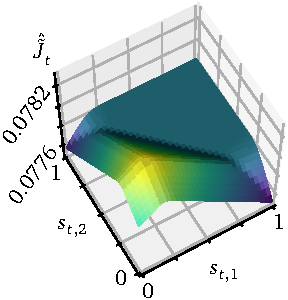
\includegraphics{financeSolution2D_1}%
  }%
  \hfill%
  \makebox[49mm][r]{%
    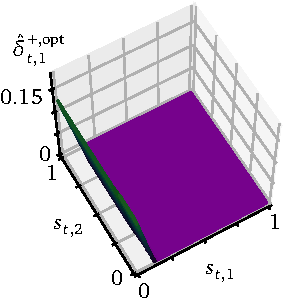
\includegraphics{financeSolution2D_2}%
  }%
  \hfill%
  \makebox[49mm][r]{%
    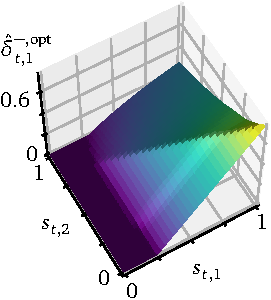
\includegraphics{financeSolution2D_4}%
  }%
  \\[0mm]%
  \makebox[49mm][r]{%
    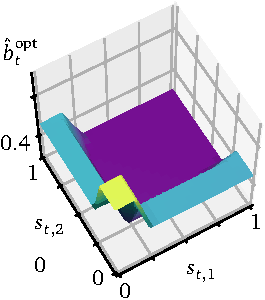
\includegraphics{financeSolution2D_6}%
  }%
  \hfill%
  \makebox[49mm][r]{%
    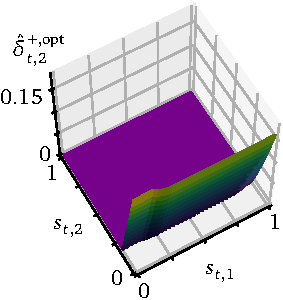
\includegraphics{financeSolution2D_3}%
  }%
  \hfill%
  \makebox[49mm][r]{%
    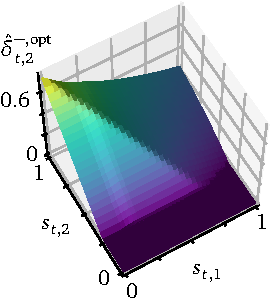
\includegraphics{financeSolution2D_5}%
  }%
  \caption[Reference solution for the two-dimensional TCP]{%
    Full grid solution for the transaction costs problem
    with $d = 2$ stocks.
    Shown are the value function $\normcetvaluefcn_t$ \emph{(top left)} and the
    optimal policy $\optnormpolicyfcn_t$ for $t = 0$.%
  }%
  \label{fig:financeSolution2DReference}%
\end{figure}

\paragraph{Convergence of the weighted Euler equation error}

\Cref{fig:financeEulerError} shows the convergence of the
$\Ltwo$ norm $\weightedeulererrorLtwo_0$ of the
weighted Euler equation error for $t = 0$ for regular sparse grids
and spatially adaptive sparse grids
for the cases of $d = 1, \dotsc, 4$ stocks.
\begin{figure}
  
\includegraphics{financeEulerError_5}%
  \\[2mm]%
  \subcaptionbox{%
    $d = 1$%
  }[37mm]{%
    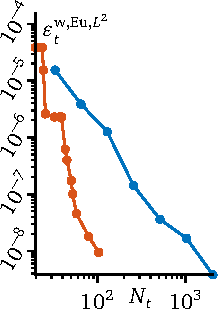
\includegraphics{financeEulerError_1}%
  }%
  \hfill%
  \subcaptionbox{%
    $d = 2$%
  }[37mm]{%
    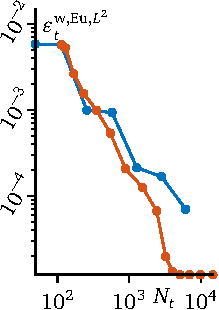
\includegraphics{financeEulerError_2}%
  }%
  \hfill%
  \subcaptionbox{%
    $d = 3$%
  }[37mm]{%
    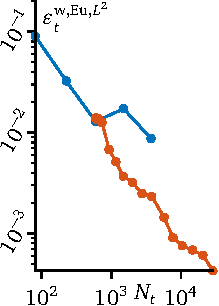
\includegraphics{financeEulerError_3}%
  }%
  \hfill%
  \subcaptionbox{%
    $d = 4$%
  }[37mm]{%
    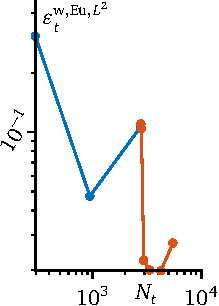
\includegraphics{financeEulerError_4}%
  }%
  \caption[Convergence of the weighted Euler equation error]{%
    Convergence of the $\Ltwo$ norm $\weightedeulererrorLtwo_t$
    of the weighted Euler equation error for $t = 0$ for
    regular sparse grids \emph{\textcolor{C0}{(blue)}} and
    spatially adaptive sparse grids \emph{\textcolor{C1}{(red)}.}
    The number $\ngp_t$ is the average number
    $\frac{1}{m_{\policy}} \sum_{j=1}^{m_{\policy}} \ngp_{t,j}$
    of grid points over all policy grids for $t = 0$,
    where $\ngp_{t,j}$ is the number of grid points
    of the $j$-th policy entry.%
  }%
  \label{fig:financeEulerError}%
\end{figure}%
For this and the following plots,
the value function grid is left unchanged
(usually a slightly refined regular sparse grid),
while the average number $\ngp_t$ of policy grid points increases
with decreasing refinement threshold $\refinetol_t$.
This is because the value function grid does not seem to have a great influence
on the convergence of the Euler equation errors.
Compared to regular grids, the spatial adaptivity decreases the error by
two orders of magnitude in one dimension.
The gain is smaller for higher dimensionalities $d$,
but spatially adaptive grids still outperform regular grids.
For $d = 2$, we observe that the error saturates
at $\ngp_t \approx \num{4000}$ points just above $10^{-5}$.
This is most likely due to the parts
\ref{item:financeErrorExtrapolation} to
\ref{item:financeErrorRounding} of the error that are not influenced
by sparse grid interpolation.
In addition, convergence significantly decelerates starting with $d = 4$.
For $d = 4$, spatially adaptive sparse grids
are able to achieve a weighted Euler equation error of
$\weightedeulererrorLtwo_t \approx \num{2.0e-2}$ for $t = 0$
(with an average number $\ngp_0 = \num{4252}$ of policy grid points).
For $d = 5$, we are still able to achieve a small error of
$\weightedeulererrorLtwo_t \approx \num{1.9e-2}$ for $t = 0$
with spatially adaptive sparse grids with
an average number $\ngp_0 = \num{12572}$ of policy grid points.
While we cannot detect any convergence for this dimensionality yet,
this is still a major result as such high-dimensional models
could not be solved up to now with conventional methods.

\paragraph{Optimal policies in 2D and 5D}

\Cref{fig:financeSolution2DSparseGrid,fig:financeSolution5DSparseGrid}
each display
\begin{figure}
  \subcaptionbox{%
    $\normcetvalueintp[1]_t$%
  }[48mm]{%
    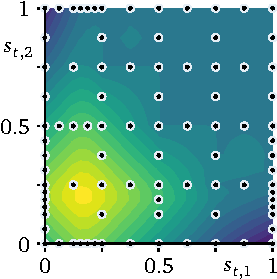
\includegraphics{financeSolution2D_7}%
  }%
  \hfill%
  \subcaptionbox{%
    $\normbuy[\opt,\sparse,1]_{t,1}$%
  }[48mm]{%
    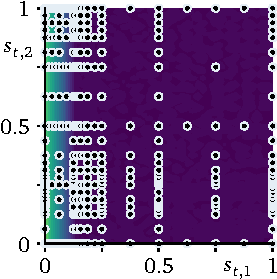
\includegraphics{financeSolution2D_8}%
  }%
  \hfill%
  \subcaptionbox{%
    $\normsell[\opt,\sparse,1]_{t,1}$%
  }[48mm]{%
    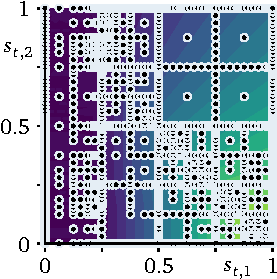
\includegraphics{financeSolution2D_10}%
  }%
  \\[2mm]%
  \subcaptionbox{%
    $\normbond_t^{\opt,\sparse,1}$%
  }[48mm]{%
    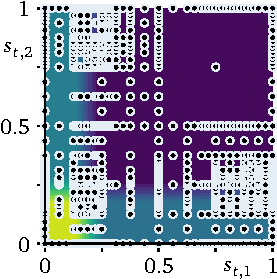
\includegraphics{financeSolution2D_12}%
  }%
  \hfill%
  \subcaptionbox{%
    $\normbuy[\opt,\sparse,1]_{t,2}$%
  }[48mm]{%
    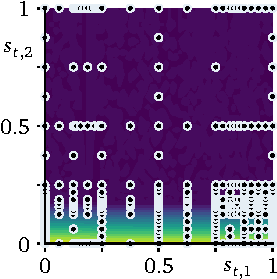
\includegraphics{financeSolution2D_9}%
  }%
  \hfill%
  \subcaptionbox{%
    $\normsell[\opt,\sparse,1]_{t,2}$%
  }[48mm]{%
    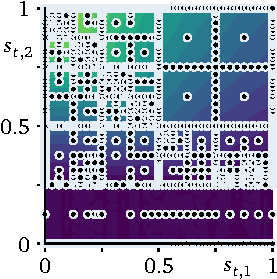
\includegraphics{financeSolution2D_11}%
  }%
  \caption[Sparse grid solution for the two-dimensional TCP]{%
    Spatially adaptive sparse grid solution for the transaction costs problem
    \vspace{-0.15em}%
    with $d = 2$ stocks.
    \vspace{-0.15em}%
    Shown are the value function $\normcetvalueintp_t$ \emph{(top left)} and the
    optimal policy $\optnormpolicyintp_t$ for the initial time step $t = 0$,
    together with the corresponding grid points \emph{(dots).}
    The color coding is the same as in
    \cref{fig:financeSolution2DReference}.%
  }%
  \label{fig:financeSolution2DSparseGrid}%
\end{figure}%
\begin{figure}
  \makebox[37mm][c]{%
    \hspace*{3.8mm}%
    \raisebox{-\height}{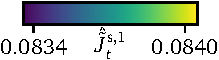
\includegraphics{financeSolution5D_13}}%
  }%
  \hfill%
  \makebox[37mm][c]{%
    \hspace*{3.8mm}%
    \raisebox{-\height}{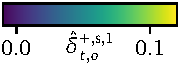
\includegraphics{financeSolution5D_14}}%
  }%
  \hfill%
  \makebox[37mm][c]{%
    \hspace*{4.4mm}%
    \raisebox{-\height}{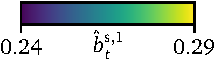
\includegraphics{financeSolution5D_16}}%
  }%
  \hfill%
  \makebox[37mm][c]{%
    \hspace*{2.4mm}%
    \raisebox{-\height}{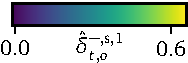
\includegraphics{financeSolution5D_15}}%
  }%
  \\[1mm]%
  \makebox[37mm][c]{%
    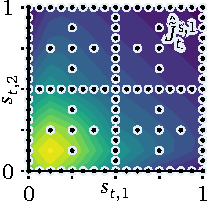
\includegraphics{financeSolution5D_1}%
  }%
  \hfill%
  \makebox[37mm][c]{%
    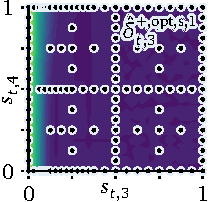
\includegraphics{financeSolution5D_4}%
  }%
  \hfill%
  \makebox[37mm][c]{%
    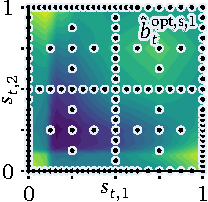
\includegraphics{financeSolution5D_12}%
  }%
  \hfill%
  \makebox[37mm][c]{%
    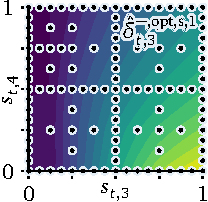
\includegraphics{financeSolution5D_9}%
  }%
  \\[1mm]%
  \makebox[37mm][c]{%
    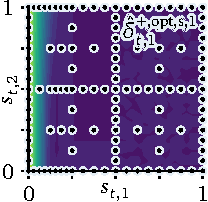
\includegraphics{financeSolution5D_2}%
  }%
  \hfill%
  \makebox[37mm][c]{%
    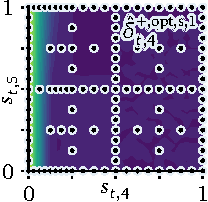
\includegraphics{financeSolution5D_5}%
  }%
  \hfill%
  \makebox[37mm][c]{%
    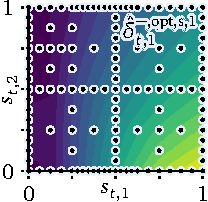
\includegraphics{financeSolution5D_7}%
  }%
  \hfill%
  \makebox[37mm][c]{%
    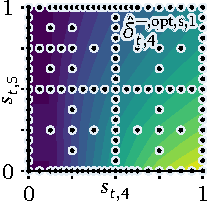
\includegraphics{financeSolution5D_10}%
  }%
  \\[1mm]%
  \makebox[37mm][c]{%
    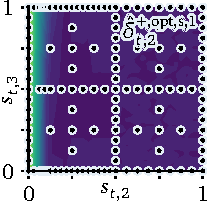
\includegraphics{financeSolution5D_3}%
  }%
  \hfill%
  \makebox[37mm][c]{%
    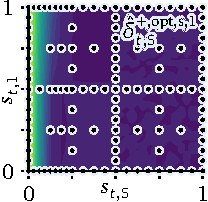
\includegraphics{financeSolution5D_6}%
  }%
  \hfill%
  \makebox[37mm][c]{%
    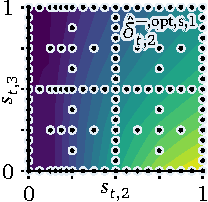
\includegraphics{financeSolution5D_8}%
  }%
  \hfill%
  \makebox[37mm][c]{%
    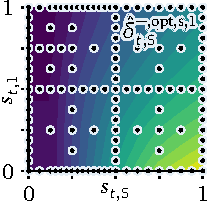
\includegraphics{financeSolution5D_11}%
  }%
  \caption[Sparse grid solution for the five-dimensional TCP]{%
    Spatially adaptive sparse grid solution for the transaction costs problem
    \vspace{-0.15em}%
    with $d = 5$ stocks.
    \vspace{-0.15em}%
    Shown are slice plots of
    the value function $\normcetvalueintp_t$ \emph{(top left)} and
    the optimal policy $\optnormpolicyintp_t$
    for the initial time step $t = 0$,
    where for each function, a pair $(o_1, o_2)$
    of dimensions to be plotted was chosen,
    and the stock fractions $\stock_{t,o}$ of the other dimensions $o$
    are set to $0.1$.
    In addition, the corresponding grid points \emph{(dots)}
    are shown as the projection onto the
    $\stock_{t,o_1}$-$\stock_{t,o_2}$ plane.%
  }%
  \label{fig:financeSolution5DSparseGrid}%
\end{figure}%
the value function and the optimal policies corresponding to
sparse grid solutions for
$d = 2$ stocks with $\ngp_0 = \num{879}$ policy grid points or
$d = 5$ stocks with $\ngp_0 = \num{12572}$ policy grid points.
Obviously, most grid points are placed along the various kinks in the
policies.
Interestingly, experiments show that the surplus-based refinement
criterion does not place more grid points along the perfectly diagonal kink
caused by the cropping of the state space
(i.e., along $\sumfcn(\vstock_t) = 1$).
It is possible to circumvent this issue by either
transforming the domain (e.g., rotations as in \cite{Bohn18Optimally}) or
directly incorporating the distance to the diagonal into the
refinement criterion for the value function.
However, we refrain from doing so here as this does not seem to
drastically improve results.
Again, this might be due to the domination of the overall error by
the parts \ref{item:financeErrorExtrapolation} to
\ref{item:financeErrorRounding} that are not related to interpolation.

\paragraph{Pointwise error}

Pointwise plots of the weighted Euler equation error
as in \cref{fig:financePointwiseError} for two stocks
reveal that there are two types of regions where the error is large:
The first type of region
is the neighborhood of the aforementioned diagonal boundary
$\sumfcn(\vstock_t) = 1$ of the uncropped region,
where the cropping distorts the error despite the weights.
The second type of region
are kinks of the optimal policy functions,
which is most visible for coarse grids
(e.g., \cref{fig:financePointwiseError_1}).
When increasing the number of grid points
(e.g., \cref{fig:financePointwiseError_1,fig:financePointwiseError_2}),
the error decreases quickly in the whole domain.

\begin{figure}
  \subcaptionbox{%
    $\ngp_t = 129$ (\num{5.3e-3})%
    \label{fig:financePointwiseError_1}%
  }[44mm]{%
    \clap{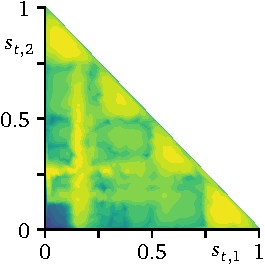
\includegraphics{financePointwiseError_1}}%
  }%
  \subcaptionbox{%
    $\ngp_t = 889$ (\num{2.1e-4})%
    \label{fig:financePointwiseError_2}%
  }[44mm]{%
    \clap{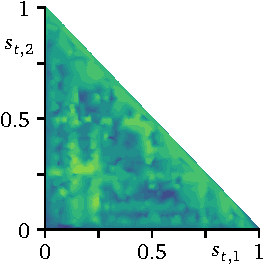
\includegraphics{financePointwiseError_2}}%
  }%
  \subcaptionbox{%
    $\ngp_t = 5159$ (\num{1.2e-5})%
    \label{fig:financePointwiseError_3}%
  }[44mm]{%
    \clap{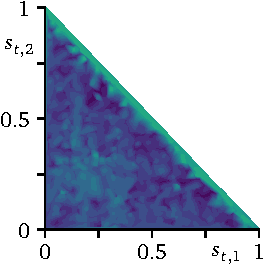
\includegraphics{financePointwiseError_3}}%
  }%
  \hfill%
  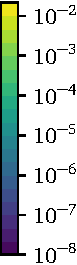
\includegraphics{financePointwiseError_4}%
  \caption[Pointwise weighted Euler equation error for different grids]{%
    Pointwise weighted Euler equation error $\weightedeulererror_t(\vstock_t)$
    ($t = 0$) for the two-dimensional transaction costs problem and
    different spatially adaptive sparse grids.
    The $\Ltwo$ error $\weightedeulererrorLtwo_t$ is given in
    parentheses.%
  }%
  \label{fig:financePointwiseError}%
\end{figure}

\paragraph{Monte Carlo simulation}

As explained in \cref{sec:828postProecessing},
we perform a multi-agent Monte Carlo simulation
and plot the resulting mean state and policy in \cref{fig:financeSimulation}
for $d = 3$, $4$, and $5$ stocks.
\begin{figure}
  
\includegraphics{financeSimulation_5}%
  \\[2mm]%
  \subcaptionbox{%
    $d = 3$ ($\ngp_0 = \num{28739}$)%
    \label{fig:financeSimulation_1}%
  }[48mm]{%
    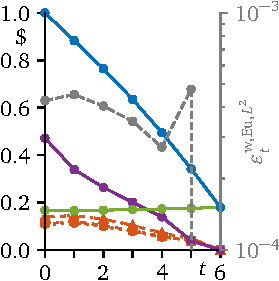
\includegraphics{financeSimulation_1}%
  }%
  \hfill%
  \subcaptionbox{%
    $d = 4$ ($\ngp_0 = \num{3343}$)%
    \label{fig:financeSimulation_2}%
  }[48mm]{%
    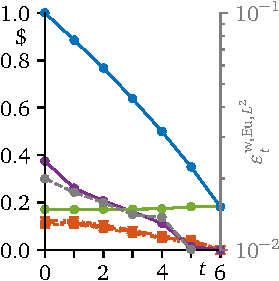
\includegraphics{financeSimulation_2}%
  }%
  \hfill%
  \subcaptionbox{%
    $d = 5$ ($\ngp_0 = \num{12572}$)%
    \label{fig:financeSimulation_3}%
  }[48mm]{%
    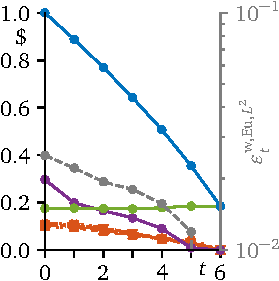
\includegraphics{financeSimulation_3}%
  }%
    \caption[Monte Carlo simulation of the TCP]{%
      Mean values of
      wealth $\wealth_t$
      \emph{\textcolor{C0}{(blue)},}
      unnormalized optimal bonds $\bond_t$
      \emph{\textcolor{C3}{(purple)},}
      unnormalized optimal consumption $\consume_t$
      \emph{\textcolor{C4}{(green)},} and
      unnormalized stock holdings
      $
        \acute{\vstock}_t
        \ceq (\vstock_t + \vnormbuy_t - \vnormsell_t) \wealth_t
      $
      after buying and selling
      \emph{\textcolor{C1}{(red)}}
      \vspace{0.1em}%
      in a Monte Carlo simulation of \num{10000} individuals,
      \vspace{-0.1em}%
      where we assume that $\wealth_0 = \$1$ for all individuals.
      In addition, the plots show the evolution of the
      $\Ltwo$ error $\weightedeulererrorLtwo_t$ over time $t$
      \emph{\textcolor{C8}{(gray, right axes)}.}%
    }%
    \label{fig:financeSimulation}%
\end{figure}%
In addition, this figure contains the evolution of the
weighted Euler equation error $\weightedeulererrorLtwo_t$ over time.
We perform a two-part assessment of the simulated results.
First, consumption should ideally be constant over time
from a finance perspective.
We measure this by calculating the coefficients of variation
(ratio of the standard deviation of the $c_t$ values to their mean),
which is \SI{2.76}{\percent}, \SI{2.68}{\percent}, and \SI{2.58}{\percent}
for $d = 3$, $4$, and $5$, respectively.
This indicates that the variation of the consumption over time
is indeed small.
Second, we consider the so-called \term{Sharpe ratios}
\cite{Sharpe66Mutual}.
The ratios are stock fractions $\vstock$ that are determined
such that the excess stock return (compared to risk-free investment)
per unit of risk is maximized:%
\footnote{%
  The Sharpe ratios per se are derived for non-skewed
  stock return rate distributions.
  Our stock return rates are log-normally distributed and thus skewed,
  but the deviation should be small after six time steps.
  However, there are variants that
  take skewed distributions into account \cite{Mueller15Ansaetze}.%
}
{%
  \setlength{\abovedisplayskip}{9pt}%
  \setlength{\belowdisplayskip}{9pt}%
  \begin{equation}
    \vecargmax_{\vstock \in \clint{0, 1}^d}
    \frac{
      \tr{\*\mu_{\range{1}{d}}} \vstock - \bondreturn
    }{
      \sqrt{\tr{\vstock} \mat{\Sigma}_{\range{1}{d},\range{1}{d}} \vstock}
    },
  \end{equation}%
}%
where $\*\mu_{\range{1}{d}}$ and
$\mat{\Sigma}_{\range{1}{d},\range{1}{d}}$
are the first $d$ entries of $\*\mu$ and
the principal minor of order $d$ of $\mat{\Sigma}$ as given in
\cref{eq:financeStockReturnMeanCovariance}.
We compare these theoretical Sharpe ratios (left)
with the simulated stock fractions
$\acute{\stock}_{t,o}/\sumfcn(\acute{\vstock}_t)$ for $t = 0$ (right):
\begin{subequations}
  \setlength{\jot}{3pt}%
  \begin{align}
    d = 3\colon\,&
    (0.314, 0.302, 0.384\rlap{),}\hphantom{, 0.999, 0.999}\quad
    (0.300, 0.317, 0.383),\\
    d = 4\colon\,&
    (0.275, 0.185, 0.250, 0.289\rlap{),}\hphantom{, 0.999}\quad
    (0.239, 0.238, 0.253, 0.270),\\
    d = 5\colon\,&
    (0.275, 0.122, 0.176, 0.203, 0.223\rlap{),}\quad
    (0.199, 0.188, 0.197, 0.205, 0.212).
  \end{align}
\end{subequations}
The simulated stock fractions
match the predicted Sharpe ratios well for $d = 3$,
while the deviation for $d \ge 4$ is larger.
However, as the simulated stock fractions do not change much over time,
we may suspect that the skewness of the distribution of the stock return rates
limits the applicability of the Sharpe ratios to these cases.

\paragraph{Complexity and computation time}

A complexity analysis reveals that the difficulty of solving
transaction cost problems quickly grows with the dimensionality $d$:
As shown in \cref{fig:structureSolveValueFunction},
the number of necessary arithmetic operations grows like
{%
  \setlength{\abovedisplayskip}{6pt}%
  \setlength{\belowdisplayskip}{6pt}%
  \begin{equation}
    \landauTheta{
      T
      \cdot \ngp_t
      \cdot \text{\#optimizer iterations}
      \cdot
      \underbrace{
        m_{\zeta}
        \cdot
        \overbrace{
          m_{\policy}
          \cdot
          \ngp_{t+1}
          \cdot m_{\state}
          \cdot p
        }^{\mathclap{\text{one evaluation of interpolant}}}
      }_{\mathclap{\text{one evaluation of objective gradient}}}\,
    },
  \end{equation}%
}%
where $m_{\state}, m_{\policy} \in \landauTheta{d}$ and
$m_{\zeta}, \ngp_t, \ngp_{t+1} \in \landauTheta{2^n n^{d-1}}$
if regular sparse grids of level $n$
without boundary points are used for state and stochastic grids
(due to $m_{\stochastic} = d$).
In addition,
the number of optimizer iterations is likely superlinear in $d$,
as this depends on the dimensionality $m_{\policy}$ of the search space
as well as on the number of multi-start points
(which also grows with $m_{\policy}$).
This means that the complexity is at least cubic in $d$,
quadratic in the average number $\ngp$ of employed state grid points, and
linear in the number $m_{\zeta}$ of quadrature points.
\Cref{fig:financeRuntime} confirms these observations with
experimental data.
\begin{figure}
  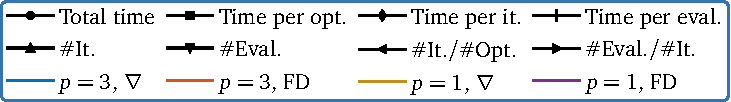
\includegraphics{financeRuntime_7}%
  \\[1mm]%
  \subcaptionbox{%
    $d = 1$%
  }[49.5mm]{%
    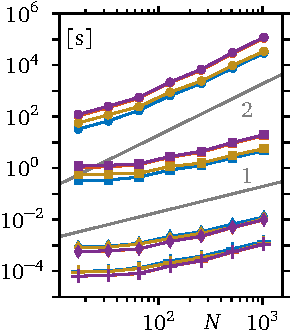
\includegraphics{financeRuntime_1}%
    \vspace*{0.3mm}\newline\hspace*{1.0mm}%
    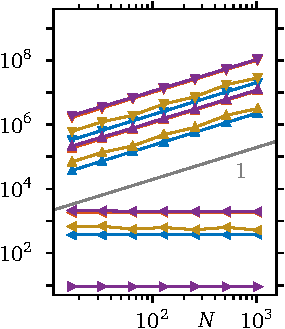
\includegraphics{financeRuntime_2}%
  }%
  \hfill%
  \subcaptionbox{%
    $d = 2$%
  }[49.5mm]{%
    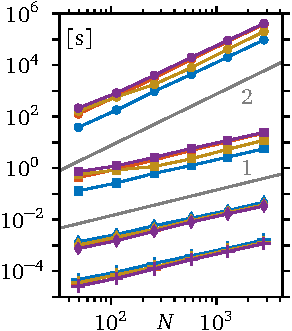
\includegraphics{financeRuntime_3}%
    \vspace*{0.3mm}\newline\hspace*{1.0mm}%
    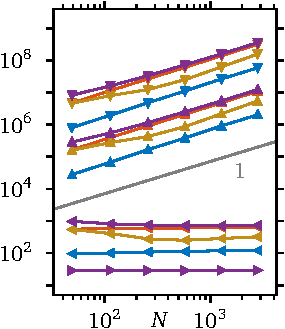
\includegraphics{financeRuntime_4}%
  }%
  \hfill%
  \subcaptionbox{%
    $d = 3$%
  }[49.5mm]{%
    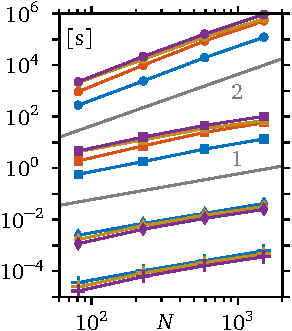
\includegraphics{financeRuntime_5}%
    \vspace*{0.3mm}\newline\hspace*{1.0mm}%
    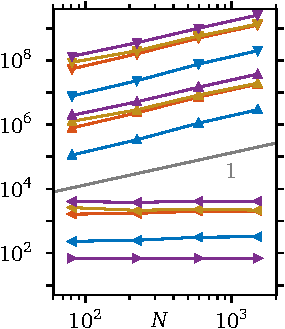
\includegraphics{financeRuntime_6}%
  }%
  \caption[Computation times and numbers of iterations for the TCP]{%
    Computation times \emph{(top)} and
    numbers of iterations and evaluations of the interpolant \emph{(bottom)}
    for the transaction costs problem on static regular sparse grids
    (i.e., without refinement).
    ``Total time'' is the serial time required to solve all
    emerging optimization problems.
    ``Time per opt.''\ is this time divided by the number
    $\mathrm{\#Opt.} = T\ngp$ of optimization problems.
    ``Time per it.''\ is the time divided by the number
    \#It.\ of optimization iterations,
    each of which is assumed to correspond to
    exactly one combined evaluation of objective function and gradient
    (the latter only if gradients are used).
    ``Time per eval.''\ is the time divided by
    the number \#Eval.\ of evaluations of
    the sparse grid interpolant and its gradient.
    The colors correspond to B-spline degrees $p = 3$ or $p = 1$ and
    to using gradients (``$\nabla$'') or finite differences (``FD'').%
  }%
  \label{fig:financeRuntime}%
\end{figure}%
For fixed $d$, the total time required by the optimization process
grows quadratically with the number $\ngp$ of grid points.
The time for one solution of the Bellman equation,
the time for one optimizer iteration, and
the time for one evaluation of the interpolant are all linear in $\ngp$,
as the number of optimizer iterations
is constant for fixed $d$.
If $d$ increases,
then the number of interpolant evaluations per optimizer iteration
(i.e., the number of quadrature points) increases as well.
Surprisingly, the number of optimizer iterations per grid point
and the time per evaluation are not monotonously increasing.
The latter observation might be due to vectorization effects.

\paragraph{Comparison to piecewise linear functions}

Hierarchical B-splines introduce two major benefits to
the solution of dynamic portfolio choice models.
The first benefit are the smooth objective functions:
When repeating the computations with piecewise linear functions (i.e., $p = 1$),
one obtains almost the same weighted Euler equation errors as in the cubic case
(except for the case of $d = 1$, where the error is one order of
magnitude greater than in the cubic case).
However, as we see in \cref{fig:financeRuntime},
the total computation time is several times larger
(e.g., more than five times for $d = 3$) for piecewise linear functions,
although evaluations are cheaper than for B-splines.
The main reason is that the number of required optimizer iterations
is for $p = 1$ almost seven times as high as in the cubic case,
since the optimizer has to deal with kinks in the objective function.
Experiments show that beginning with $d = 4$,
the total optimization time required to solve the transaction costs problem
is one whole order of magnitude shorter for cubic B-splines
than for piecewise linear functions.

\paragraph{Comparing exact gradients to finite differences}

The second benefit is the availability of exact gradients:
\Cref{fig:financeRuntime} also contains computation times of the
solution process
if we artificially do not use exact gradients of the objective functions,
but rather approximate them with finite differences.
For each evaluation of the objective gradient,
at least $m_{\policy}$ additional evaluations of the objective function
have to performed to compute the finite differences
($2m_{\policy}$ if central differences are used).
Consequently, while the resulting weighted Euler equation errors are
similar, the total optimization time roughly increases by a
factor of up to five if we do not use exact gradients.


\cleardoublepage
